\documentclass[3p,times,12pt]{elsarticle}

\usepackage{multirow}
\usepackage{booktabs}
\usepackage[utf8]{inputenc}
\usepackage{blindtext}
\usepackage{graphicx}
\usepackage[flushleft]{threeparttable}
\usepackage{lscape}
\usepackage{float}
\usepackage{appendix}
\usepackage{hyperref}
\usepackage{siunitx}
\usepackage{colortbl}
\usepackage{enumitem}
\usepackage{makecell}
\usepackage{xurl}
\usepackage{natbib}
\renewcommand\theadfont{\bfseries}

\usepackage{lineno}
\usepackage[utf8]{inputenc}
\usepackage{array}
\usepackage{wrapfig}
\usepackage{tabularx}
\usepackage{caption}
\usepackage{booktabs}
% \usepackage{amssymb}
\usepackage{amsmath}
% \usepackage{bbding}
\usepackage{tikz}
\usepackage{xcolor}
\usepackage[figuresright]{rotating}
\usepackage{tablefootnote}
\usepackage{color}
\usepackage{tabularray}
\usepackage{orcidlink}
% \usepackage[demo]{graphicx}
% \usepackage{subfig}


\def\halfcheckmark{\tikz\draw[scale=0.4](0,.35) -- (.25,0) -- (1,.7) -- (.25,.15) -- cycle (0.75,0.2) -- (0.77,0.2)  -- (0.6,0.7) -- cycle;}
\def\fullcheckmark{\tikz\fill[scale=0.4](0,.35) -- (.25,0) -- (1,.7) -- (.25,.15) -- cycle;} 

\biboptions{sort&compress}
\captionsetup[table]{justification=raggedright,singlelinecheck=off}

\biboptions{sort&compress}
\journal{Building Simulation}

\begin{document}
\begin{sloppypar}

\begin{frontmatter}


\title{Evaluating Different Levels of Information on the Calibration of Building Energy Simulation Models}

% ----------------------------------------------------------------------------
% \author[nus]{Siyu Cheng\orcidlink{0000-0002-4133-5507}}
% \author[nus]{Zeynep Duygu Tekler\orcidlink{https://orcid.org/0000-0002-1858-0846}}
% \author[cqust]{Hongyuan Jia\orcidlink{0000-0002-0075-8183}}
% \author[seu]{Wenxin Li\orcidlink{0000-0001-9866-6713}}
% \author[nus]{Adrian Chong\corref{mycorrespondingauthor}\orcidlink{0000-0002-9486-4728}}
% \cortext[mycorrespondingauthor]{Corresponding author}
% \ead{adrian.chong@nus.edu.sg}

% \address[nus]{Department of the Built Environment, College of Design and Engineering, National University of Singapore, 4 Architecture Drive, Singapore 117566, Singapore}

% \address[cqust]{School of Civil Engineering and Architecture, Chongqing University of Science and Technology, Chongqing, 401331, China}

% \address[seu]{School of Energy and Environment, Southeast University, Nanjing 210096, China}
% ----------------------------------------------------------------------------
\begin{abstract}
A poorly calibrated model undermines confidence in the effectiveness of building energy simulation, impeding the widespread application of advanced energy conservation measures (ECMs). Striking a balance between information-gathering efforts and achieving sufficient model credibility is crucial but often obscured by ambiguities. To address this gap, we model and calibrate a test bed with different levels of information (LOI). Beginning with an initial model based on building geometry (LOI 1), we progressively introduce additional information, including nameplate information (LOI 2), envelope conductivity (LOI 3), zone infiltration rate (LOI 4), AHU fan power (LOI 5), and HVAC data (LOI 6). The models are evaluated for accuracy, consistency, and the robustness of their predictions. Our results indicate that adding more information for calibration leads to improved data fit. However, this improvement is not uniform across all observed outputs due to identifiability issues. Furthermore, for energy-saving analysis, adding more information can significantly affect the projected energy savings by up to two times. Nevertheless, for ECM ranking, models that did not meet ASHRAE 14 accuracy thresholds can yield correct retrofit decisions. These findings underscore equifinality in modeling complex building systems. Clearly, predictive accuracy is not synonymous with model credibility. Therefore, to balance efforts in information-gathering and model reliability, it is crucial to 1) determine the minimum level of information required for calibration compatible with its intended purpose and 2) calibrate models with information closely linked to all outputs of interest, particularly when simultaneous accuracy for multiple outputs is necessary.

% Our results indicate that higher levels of information were not always essential for retrofit analysis. Additionally, we show that a model with a high CV(RMSE) value may not always mean that a model is not good enough for its intended purpose. In contrast, a low CV(RMSE) may not always indicate a good model due to identifiability issues because existing calibration approaches are overparameterized by design. 

\end{abstract}

\begin{keyword}
calibration \sep building energy simulation (BES) \sep energy conservation measure (ECM) \sep level of information \sep field measurements
\end{keyword}
% Model fidelity \sep 

\end{frontmatter}

\newcommand{\tabincell}[2]{\begin{tabular}{@{}#1@{}}#2\end{tabular}}
\newcolumntype{L}[1]{>{\raggedright\arraybackslash}p{#1}}
\newcolumntype{C}[1]{>{\centering\arraybackslash}p{#1}}
\newcolumntype{R}[1]{>{\raggedleft\arraybackslash}p{#1}}
\newcommand{\RNum}[1]{\uppercase\expandafter{\romannumeral #1\relax}}

\section{Introduction}
\label{S:1} 
According to the International Energy Agency (IEA) \cite{iea2022}, buildings accounted for 30\% of global final energy consumption and 27\% of total energy sector emissions in 2021. The absence of widespread decarbonization of existing buildings will continue to perpetuate emissions from the building stock, impeding the achievement of the 1.5$^{\circ}$C target outlined in the Paris Climate Agreement \cite{iea2020energy}. To mitigate climate change, energy retrofits and the implementation of energy conservation measures (ECMs) have emerged as effective solutions for reducing energy consumption in buildings. Projections indicate that by 2030, building energy use could be reduced by over 20\% using cost-effective technologies, while deep retrofits could achieve reductions of more than 35\% \cite{doe2015assessment}. BES is increasingly being used to support the design and retrofit of buildings. Consequently, the importance of accurate and efficient building energy simulations (BES) to predict the influence of different building designs on energy performance remains a top concern. 

The U.S. Department of Energy (DOE) defines building energy simulation as a simulation program that uses physics-based equations and various inputs to calculate building energy use, along with related metrics like occupant comfort and energy costs \cite{DOE2018BEM}. Some examples of these inputs include weather information, geometry, construction materials, internal loads, HVAC systems, operational schedules, control strategies, and thermostat settings. However, it is important to recognize that a simulation model is not an exact replica of a mathematical model nor a perfect representation of the physical building, especially when the physics are not fully resolved \cite{mehta2016simulation}. There are also many uncertainties that influence a model's ability to reflect actual building performance accurately \cite{{van2016review}}. These uncertainties in modeling processes can result in deviations between measured and simulation data. As reported in a study on energy performance for 121 LEED new construction buildings \cite{turner2008energy}, there are notable discrepancies between simulated and measured energy use intensity, and over half the projects surveyed deviate by more than 25\% from the simulation projections during the design phase. To accomplish a better fit between the time series, calibration is typically carried out to match simulation predictions to measured data and reduce uncertainties in the model.

Building energy model calibration is the process of characterizing the unknown parameters to minimize the discrepancy between the prediction and the reality. In general, calibration approaches can be divided into manual or automated calibration \cite{coakley2014review}. Automated calibration utilizes computerized processes to tune model parameters, with the objective of maximizing the model's fit to observations. In contrast, manual calibration relies on iterative pragmatic intervention by the modeler to iteratively adjust input parameters until simulation outputs match actual measurements. According to a recent review on BES calibration \cite{chong2021calibrating}, 66\% of the reviewed papers use automated calibration approaches, which has approximately tripled when compared to the 26\% in a 2014 review by \citet{coakley2014review}. Typical automated calibration approaches include Bayesian calibration \cite{heo2011bayesian, chong2018guidelines, chong2019framework}, pattern-based approach \cite{sun2016pattern, sun2022application}, and optimization-based approach \cite{robertson2013evaluation, hong2017automatic, asadi2019building, zhang2020development}. In terms of manual calibration, continuous efforts have been devoted to establishing formal and systematic manual calibration approaches, such as evidence-based calibration \cite{coakley2011calibration, raftery2011evidence, raftery2011detailed, bertagnolio2012evidence, yin2016linking, mihai2017bottom, da2021evaluation}, multi-stage calibration \cite{cacabelos2017development, zuhaib2019application, pachano2021multi}, and simultaneous multi-level calibration \cite{yang2015model}.

Although the effectiveness of the above calibration approaches has been demonstrated in specific proof-of-concept settings, the non-identifiability issue, which refers to the difficulty of identifying the true values of a model’s calibration parameters, remains unsolved \cite{arendt2012improving, menberg2017efficiency, chong2018guidelines}. 
The complexity of whole building energy modeling, coupled with limited information available for parameter estimation, is the root of the identifiability problem. This results in a vast and under-determined parameter space, and thus, different combinations of parameters could achieve similar magnitudes of prediction errors \cite{Zhan2023sep}. It has been highlighted that lower errors do not necessarily indicate better parameter estimation \cite{angelotti2023calibrating}. Many studies underscore the need to reduce uncertainty in the model's input parameters. \cite{scortegagna2023can} conducted deterministic and stochastic simulations, revealing that the ground truth lies within an uncertainty range defined by variability in model input parameters. This outcome suggests that the calibrated model is just one among many alternatives that yield simulated outputs closely aligned with measured values. Consequently, achieving a credible calibration for a building energy simulation model is challenging without access to more accurate measurements and comprehensive information about reality. \cite{ekstrom2021evaluating} demonstrated the substantial impact of parameter uncertainty on the model's predicted results. Their findings indicate that data quality significantly alters probability density curves, thereby influencing the accuracy of energy performance predictions. Moreover, \citet{risch2021influence} reported that calibration with more information resulted in less error compared to using a low level of information. Therefore, there is a crucial need to facilitate access to real building performance data and enhance measurement accuracy and granularity. In an early study, \citet{bertagnolio2012evidence} argued that the use of a fully automated method to solve the highly under-determined calibration problem could lead to erroneous parameter estimation and deviations between simulation and real building performance. The author thus suggested considering each parameter one after the other and sticking to a systematic, evidence-based approach. Generally, the goal of model calibration is to eliminate uncertainties in model inputs. Considering the importance of input information for this purpose, it is necessary to bring evidence-based decision-making to the calibration process.  

Evidence-based calibration is a multi-stage sequential approach that gives priority to the physical identification of the model’s parameters (i.e., to the direct measurement) and relies on the notion of hierarchy among the source of information to identify the value of the parameters \cite{bertagnolio2012evidence}. The order of the information in the hierarchy is subject to the (estimated) reliability of the source of information. Unlike automated approaches that usually rely on mathematical and statistical techniques, evidence-based calibration only makes changes to the input parameter based on available information under clearly defined priorities. It prioritizes the information gained from measurement and direct observation. Driven by the increased availability and quality of information, the simulation models' capability for representing real building operations can be enhanced throughout the sequential calibration process.

The hierarchy of information sources forms the basis for classifying calibration levels. \citet{reddy2006literature} proposed a five-level calibration based on the availability and reliability of the source of information: the first level involves information from as-built drawings and design specifications, constituting the "as-built" model. The second level incorporates site visits and cross-verification into the "as-built" model. The third level adds detailed audits and spot measurements. The fourth level introduces short-term monitoring with data loggers. The fifth level involves long-term monitoring. Building on these levels, \citet{bertagnolio2012evidence} applied the first, second, and fourth levels of calibration to a 10,100 $m^2$ building, and \citet{mustafaraj2014model} explored the second and fifth levels using a three-story 4500 m2 building in Ireland. \citet{raftery2011evidence} integrated a process for investigation of further measurement with the sequential evidence-based calibration framework, developing an iterative calibration process. This approach can identify additional measurements to minimize discrepancies between simulated and actual energy performance. Using this, the Coefficient of the Variation of the Root-Mean Square Error (CV(RMSE)) for monthly total electricity dropped from 79.26\% to 1.35\%, and hourly CV(RMSE) plunged from 94.02\% to 1.87\%. \citet{zuhaib2019application} proposed a similar framework. The framework was evaluated using a case study, giving a 15\% CV(RMSE) for monthly total electricity consumption and a 17\% CV(RMSE) for hourly indoor air temperature prediction. Overall, these studies demonstrate the improvement of model accuracy across different levels of calibration. However, the question of how the level of information affects the model's predictive performance for its intended use still remains unanswered in both the literature and current guidelines \cite{guideline200214, united2001international, femp2015m}. 

Another challenge in calibrating building energy models concerns the disconnection between the evaluation metrics and the model's intended use. Current calibration studies rely solely on accuracy metrics to assess a model's calibration performance. Among these metrics, the Coefficient of the Variation of the Root Mean Square Error (CV(RMSE)) and Normalized Mean Bias Error (NMBE) are mostly used as they are specified by ASHRAE Guideline 14 \cite{guideline200214}, the International Performance Measurement and Verification Protocol (IPMVP) \cite{united2001international}, and the Federal Energy Management Program (FEMP) \cite{femp2015m}. However, these metrics may not provide reliable guidance due to their absolute values being detached from the simulation's purpose \cite{chong2021calibrating}.
Consequently, \citet{reddy2007calibrating} points out that comparison between measured and predicted performance should be seen not in terms of whether the program agrees with the measurements but whether the program is good enough for its intended purpose. 

In the spirit of Occam’s razor, which advocates the principle of parsimony in model development, considerable efforts have been devoted to parsimonious modeling. This modeling approach aims to find the most appropriate model that meets the simulation objectives with minimal complexity \cite{tuysuz2020calibrating}. For instance, \citet{gaetani2016occupant} evaluated the impact of occupant behavior on building energy performance. They proposed a fit-for-purpose framework to select the best approach for modeling occupant behavior for energy simulation at the building scale. \citet{mathur2020towards} examined the effect of extended Level of Detail (LoD) on urban building energy modeling, highlighting the significant effect of the occupancy schedule profile and the minimal impact of other parameters. \citet{saad2023investigating} investigated the effect of different geometrical methods, model complexity, and building characteristics data sources on the model's performance to identify fit-for-purpose guidelines for developing urban building energy models. \cite{hu2023impacts} explored the impact of building load profile characteristics on the model's load forecast accuracy. The findings indicate that for buildings with a low load dispersion level, a simple model can demonstrate satisfactory performance for the design, control, and fault diagnosis of building energy systems. These studies highlight the opportunities to tailor modeling and calibration approaches to the intended purpose of simulation while simultaneously achieving satisfactory predictive performance with a minimal level of information. However, due to the absence of consensus guidance on how to qualify the reliability of a building energy model for various applications, the assessment of calibration performance relies solely on accuracy-based metrics in many existing studies, with identical thresholds applied to diverse observed outputs. The over-reliance on accuracy may bias the selection of models and calibration approaches. It also raises questions about whether the achieved accuracy is sufficient and essential for a specific simulation purpose. Therefore, the evaluation of the model and calibration approach should not be separated from the intended purpose of the simulation. Besides, more emphasis should be attached to context-based metrics, such as ECM ranking or estimated energy savings for retrofit analysis. 

In summary, detailed energy simulation programs typically involve numerous input parameters, resulting in large parameter space and non-identifiability issues that have not been addressed in building energy model calibration studies. Calibrating against a single output using less information requires less effort for information gathering but could increase model bias or inadequacy. A poorly calibrated model undermines confidence in the effectiveness of building energy simulation, impeding the widespread application of advanced energy conservation measures (ECMs). In contrast, incorporating higher-level information in calibration can reduce the parameter space and consequently enhance identifiability and accuracy but tends to be more data and computationally intensive. Striking a balance between information-gathering efforts and achieving sufficient model credibility is crucial but often obscured by ambiguities. Therefore, it is necessary to identify a reasonable level of information for model calibration to meet the simulation objectives while considering the data acquisition effort. However, current guidelines \cite{guideline200214, united2001international, femp2015m} overlook the information requirement for calibration. There are no guidelines on data requirements for model calibration using detailed simulation programs. Although some literature, such as \cite{bertagnolio2012evidence, lim2018influences, derakhti2022impact}, investigated the influences of the selection of information or energy data for calibration on calibration error indexes. These studies focused on model accuracy only. None of them looked at the impact of different levels of information on the model's credibility for predictions. This underscores the need for a more in-depth understanding of the impact of different levels of information on calibration, especially on its predictive performance for a specific context of use. 
To fill this gap, this study applied the evidence-based sequential calibration approach to a test bed to demonstrate the impact of the level of information on model accuracy and its predictive performance. The objectives of this study are to:

\begin{itemize}
    \item Examine how an additional level of information enhances the data fit within the framework of ASHRAE Guideline 14 \cite{guideline200214}; 
    \item Quantify the impact of different levels of information on calibration performance for retrofit analysis, particularly in terms of ECM ranking and energy-saving predictions;
    \item Demonstrate the importance of calibration for obtaining a reliable model that is compatible with its intended purpose;
    \item Determine the appropriate level of information needed to adequately calibrate a model for retrofit analysis.
\end{itemize}


\section{Method}
\label{S:2}

\subsection{Overview} 
\label{S:2.1}
Figure \ref{fig:testbed} depicts the layout of the testbed (measuring $5.7m \times 4.3m \times 2.6m$). It was selected as the studied case to quantify the impact of the increased amount of information on building energy model calibration and its predictive performance. Figure \ref{fig:framework} illustrates the overall workflow of the case study, which consists of five steps:  
1) data acquisition, 2) evidence-based model improvement, 3) simulation-based ECM analysis, 4) model evaluation, and 5) robustness analysis). 

\begin{figure}[H]
\centering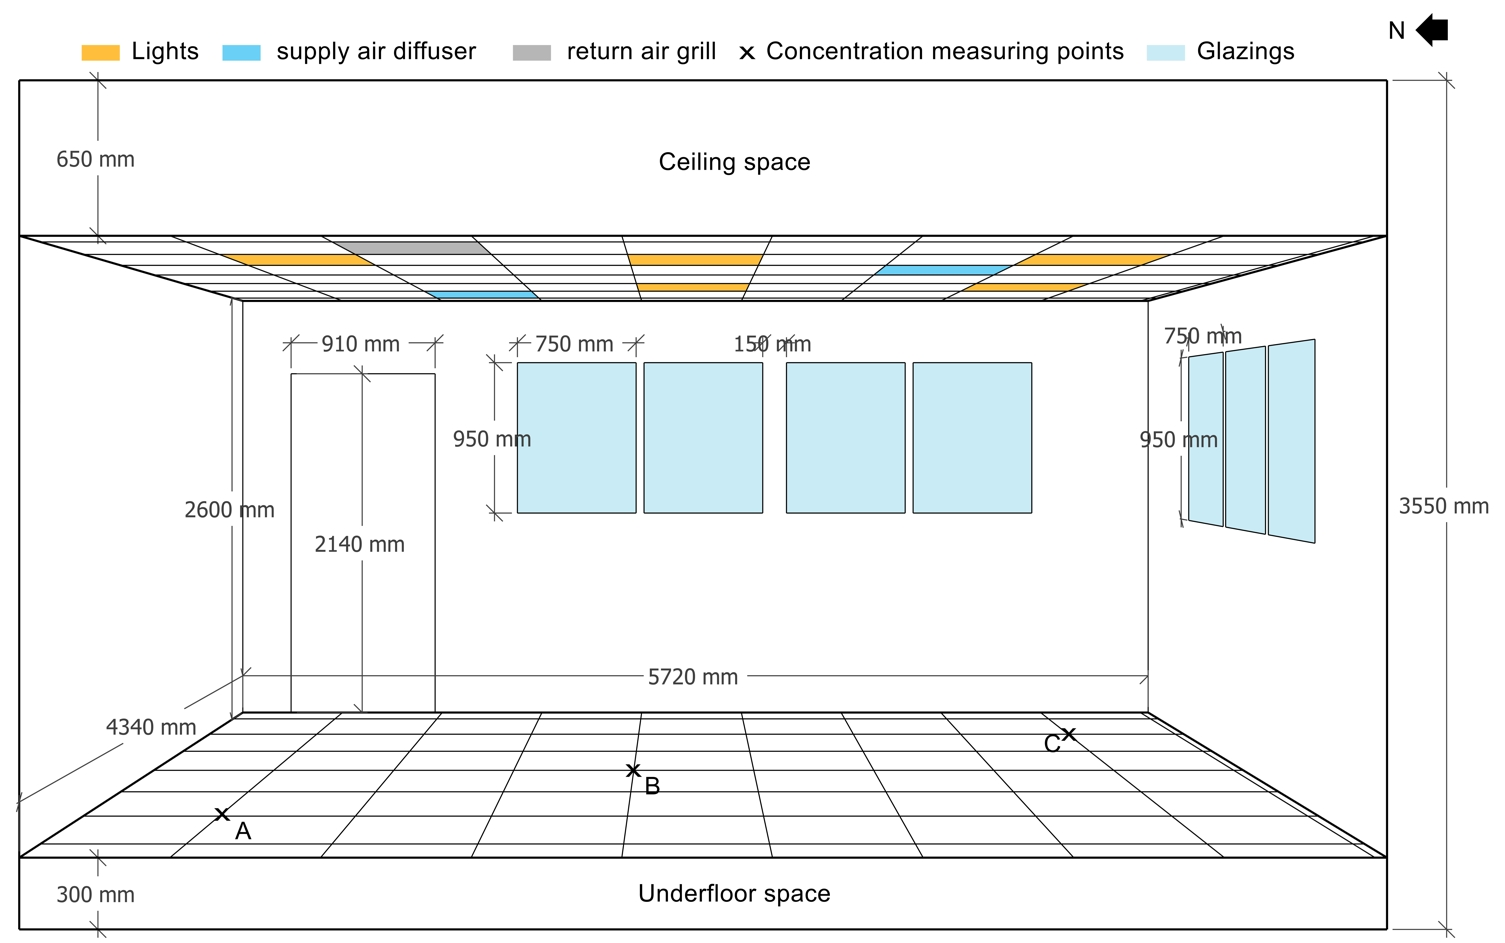
\includegraphics[width=1\linewidth]{pic/sbb_geometry_4.jpg}
% \centering\includegraphics[width=1\linewidth]{pic/testbedSBB3.jpg}
\caption{Layout of the test bed}
\label{fig:testbed}
\end{figure}

As shown in the workflow Figure \ref{fig:framework}, six levels of information (LOI) were developed according to the information and on-site measurements available for the studied case. LOI 1 corresponds to the initial model (Model 1). Starting from the initial model, each level of information was added to the initial model to develop a set of models:

\begin{itemize}
\item \textit{Model 1:} developed from LOI 1: as-built drawings, including architectural, electrical, HVAC, and other systems, providing an accurate representation of the system design, dimensions, and zonings. The unknown parameters are defined using the default simulation program template and the modeler's best-informed assumptions.
\item \textit{Model 2:} developed from Model 1 + LOI 2: design specifications and site verification through nameplate inspection and interviewing of the building operator. Envelope thermal properties are defined according to design specifications. The system size, chilled water supply temperature (CHWT), fan nominal power, Variable Air Volume terminal's design air flow rate, Air Handling Unit nominal capacities, etc., are defined according to physical nameplate inspection and operator interviews.
\item \textit{Model 3:} developed from Model 2 + LOI 3: measurements on envelope thermal conductance using heat flow meter method (refer to Section \ref{S:2.2.1}).
\item \textit{Model 4:} developed from Model 3 + LOI 4: measurements on zone infiltration rate using concentration decay method (refer to Section \ref{S:2.2.2}).
\item \textit{Model 5:} developed from Model 4 + LOI 5: Fan in-site performance measurement (refer to ASHRAE Guideline 15 Annex A4.2 Equipment Testing Standards: Fans)
\item \textit{Model 6:} developed from Model 5 + LOI 6: HVAC system temp, flow, and thermal energy measurements using existing Building Management System (BMS).
\end{itemize}

The application of the evidence-based process (LOIs 1 to 5) significantly reduced the dimension of the calibration problem. Model 5 represents the last evidence-based step in the frame of this study. An iterative adjustment was performed in Model 6, serving as a final resort to refine the calibration of the model. This step involved tuning values for influential but not easily measurable parameters, such as the return air ratio in this study. To facilitate reproducibility, we have established a GitHub repository\footnote{https://github.com/ideas-lab-nus/sbb-calibration} containing the necessary resources for reproducing the calibration process and replicating this research.

\begin{figure}[H]
\centering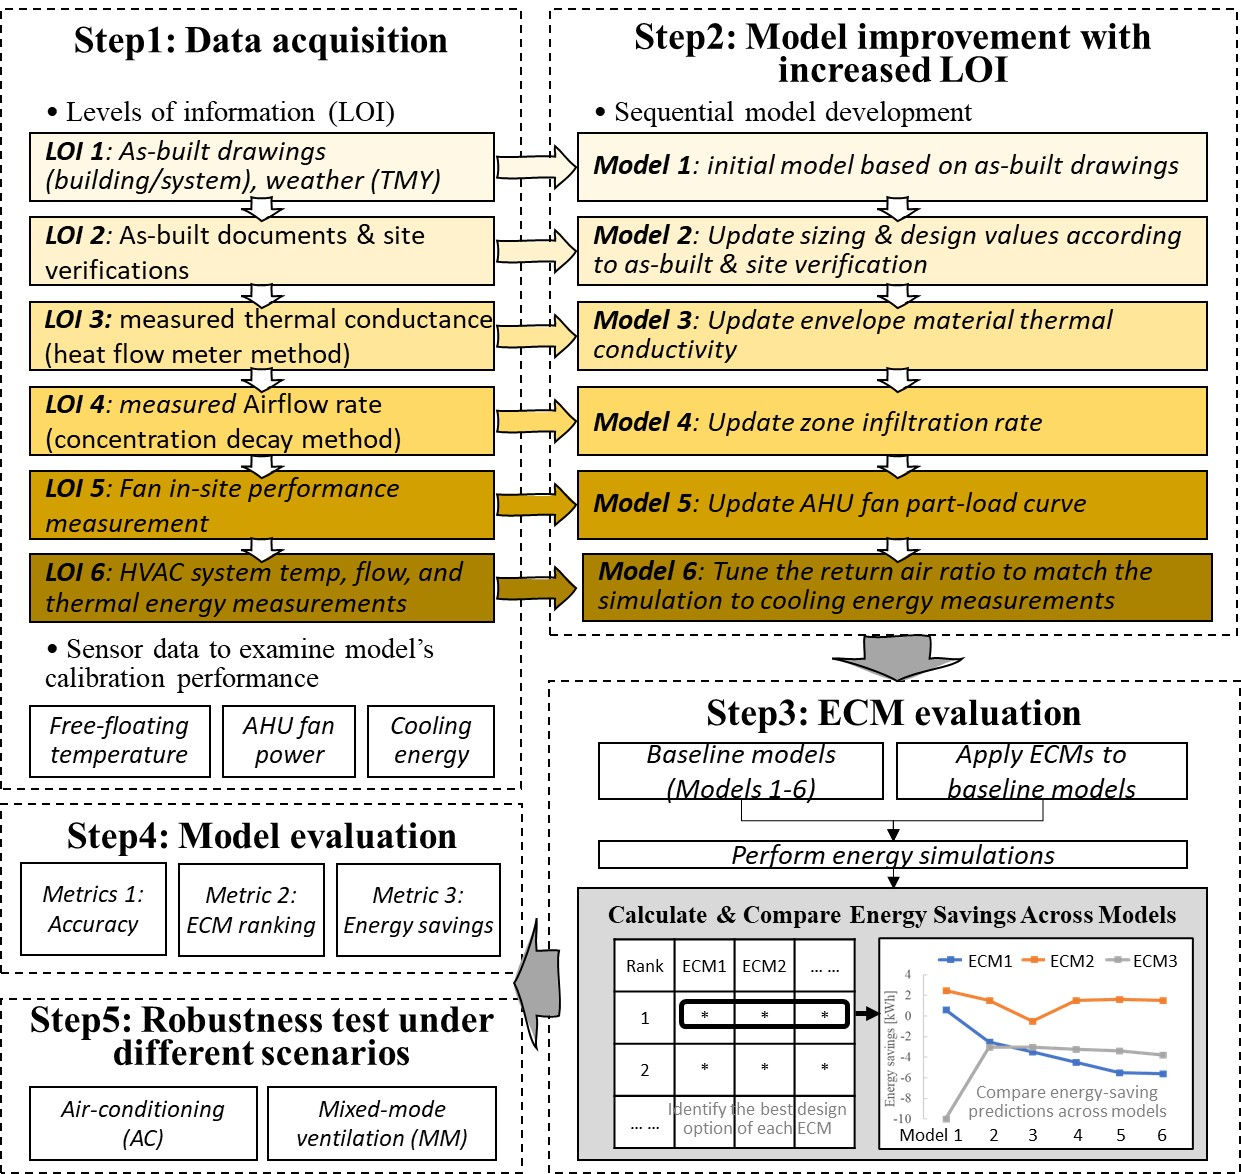
\includegraphics[width=0.95\linewidth]{pic/framework_7.jpg}
\caption{Proposed framework to quantify the impact of different levels of information on the predictive performance for retrofit analysis}
\label{fig:framework}
\end{figure}

\subsection{Data acquisition}
\label{S:2.2}
In this section, we describe the measurement protocols undertaken to acquire the data used in this study to calibrate the model. A series of experiments were conducted to gather the measured data, which serves as more reliable information in the hierarchy. The data was subsequently used for parameter estimation to update the model sequentially. The measurements were carried out as follows. 

\begin{itemize}
\item Thermal resistance measurement (3 days): This test measured the thermal resistance of the building envelope components, contributing to Level 3 information;
\item Airflow rate measurement (1 day): This test measured the zone air infiltration rate for Level 4 information;
\item Fan characterization tests (1 day): This test gathered the supply fan's power consumption at different fan speeds, contributing to Level 5 information;
\item HVAC tests (6 days): This test gathered the hourly data from BMS, especially the supply air temperature, supply air flow rate, and the AHU cooling coil cooling energy consumption under different setpoints, corresponding to Level 6 information. 
\end{itemize}

Apart from the above measurements, a free-floating test (2 days) was conducted to gather data for evaluating the building's calibration performance during non-operating hours. Hourly-based zone temperature and relative humidity were gathered. During the free-floating test, there are no internal loads (in particular occupancy), and the HVAC system is turned off so that we can measure the envelope thermal properties and infiltration rates more reliably without potential confounders. Table \ref{tab:sensors} summarizes the sensors used and their corresponding accuracy. 

\begin{table}[H]
\centering
% \small
\scriptsize
% \footnotesize
\caption{Technical specifications and accuracy}
\label{tab:sensors}
\resizebox{\textwidth}{!}{%
\begin{tabular}{L{3cm} C{1cm} C{1cm} L{6cm}}
\toprule
Sensor & Accuracy & Unit & Measured variable \\
\midrule
Anemometer & ± 3\% & m/s & Air velocity inside rooms \\
Temperature sensors & ± 0.2 & °C & Surface temperatures, air temperature \\
RH sensors & ± 3\% & \% & Relative humidity inside and outside \\
Heat flux sensors & ± 2\% & $W/m^2$ & Heat flux through surfaces \\
Power meter & ± 1\% & W & Input power of the electric heaters and artificial lights \\
\multicolumn{1}{m{3cm}}{Innova 1312 photoacoustic multi-gas analyser} & 0.001 & ppm & SF6 concentrations \\
Building management system (BMS) & & & \multicolumn{1}{m{6cm}}{It is instrumented with high-quality sensors that measure all relevant parameters, such as temperature and relative humidity, air flow rate \& temperature, ON/OFF and modulating damper, fan static pressure, CO2 concentration, thermal energy, and electric power} \\
\bottomrule
\end{tabular}%
}
\end{table}

\subsubsection{Thermal resistance test}
\label{S:2.2.1}
Thermal resistance was measured using the heat flow meter method, conducted in accordance with the ISO 9869-1:2014 standard \cite{iso20149869}. Figure \ref{fig:RTD_HFM} illustrates the placement of thermocouples at the center of each exterior and interior envelope surface, while heat flow meters were positioned at the center of each inside surface. An averaging method was employed to calculate the thermal resistance of each envelope component. Before calculating the thermal conductance, two conditions were verified: 1) the duration of the test exceeded 72 hours, and 2) the R-value obtained at the end of the test did not deviate by more than ± 5\% from the value obtained 24 hours before.

\begin{figure}[H]
\centering\includegraphics[width=0.8\linewidth]{pic/RTD_HFM.jpg}
\caption{Installment of the temperature and heat flow meters}
\label{fig:RTD_HFM}
\end{figure}

\subsubsection{Zone infiltration rate test}
\label{S:2.2.2}
Zone infiltration was measured using the tracer gas decay method following the ISO 12569-2017 standard \cite{iso12569}. Specifically, SF\textsubscript{6} concentrations were sampled and measured using an INNOVA 1312 photo-acoustic multi-gas analyzer and an INNOVA 1309 multi-channel sampler. The tracer gas source was placed at the center of the test room. Three sampling points (points A-C, as shown in \ref{fig:testbed}) were strategically placed at the room center and two corners to measure SF\textsubscript{6} concentration at the height of 1.1m from the ground. Three fans were placed upstream of the tracer gas injection lines to spread the gas more evenly before sampling started. The steps are as follows: First, inject the tracer gas for 5 seconds, mix the tracer gas by using the fan, and check the uniformity of concentration in the space with obtained samples of the initial condition. Then, wait for the analyzer to receive air from all sampling points through a multiplexer programmed at 1-minute intervals. SF\textsubscript{6} concentrations at the three sampling points were thereby sampled approximately every 3 minutes during the concentration decay process. Next, check the uniformity of concentration in the zone with obtained samples before stopping the measurement. At last, plot the obtained samples in graph $\ln\left(N\right)$ versus $t$ and calculate the specific airflow rate ($N$) using Equation \ref{eq:ach1}. Equation \ref{eq:ach2}) is transformed from Equation \ref{eq:ach1} when the specific airflow rate does not fluctuate over time and there is a linear relationship between $\ln\left(N\right)$ and $t$. These values were plotted in Figure \ref{fig:decay}, where the natural log of the measured SF6 concentration data was subjected to linear regression to calculate the infiltration rate. The measured air infiltration rates, determined by the absolute value of the slope, were 0.0424, 0.0438, and 0.0410 air changes per hour (ACH) for locations at points A, B, and C, respectively. 

\begin{equation}
\label{eq:ach1}
\bar N = \frac{1}{{t}_{2}-{t}_{1}} \log_{e}{\frac{C\left({t}_{1}\right)}{C\left({t}_{2}\right)}}
\end{equation} \\
where \\
$\bar N$ is the mean time-specific airflow rate, in $1/h$ or $1/s$; \\
$C\left({t}_{1}\right)$ \quad is the room concentration at ${t}_{1}$, in $m^3/m^3$. \\
$C\left({t}_{2}\right)$ \quad is the room concentration at ${t}_{2}$, in $m^3/m^3$. \\
${t}_{1}$ \qquad is the start point of measurement in h. \\
${t}_{2}$ \qquad is the end point of measurement in h. \\

\begin{equation}
\label{eq:ach2}
log_{e}{C\left(t\right)} = log_{e}{C\left({t}_{1}\right)} - N\left(t-{t}_{1}\right)
\end{equation} \\
where \\
$N$ \qquad is the specific airflow rate, in h.\\
$C\left(t\right)$ \quad is the room concentration at $t$, in $m^3/m^3$. \\
${t}_{1}$ \qquad is the start point of measurement, in h. \\

\begin{figure}[H]
    \centering
    \includegraphics[width=1\linewidth]{pic/decay_test.jpg}
    \caption{The concentration decay curve at three sampling points}
    \label{fig:decay}
\end{figure}

\subsubsection{Measurement uncertainty analysis}
\label{S:2.2.3}

Errors and uncertainties can arise from three sources: sampling, modeling, and measurement. IPMVP (International Performance Measurement \& Verification Protocol) \cite{IPMVP2012} provides a comprehensive introduction to uncertainty calculation. We refer to the IPMVP Appendix B \cite{IPMVP2012} and the National Physical Laboratory's Guide to Uncertainty of Measurement (NPL Guide) \cite{bell2001beginner} for uncertainty calculation. The included uncertainty components in this study are listed as follows:

\begin{enumerate}
    \item The standard error of the sample mean (refer to IPMVP Appendix B-1.3 and NPL Guide Section 3.6). 
    \item The standard error of regression coefficients (refer to IPMVP Appendix B-2.2.3).
    \item The standard error of the measured value (refer to IPMVP Appendix B-4 and \cite{taner2015optimisation}).
    \item Combining standard errors. The calculation for combined uncertainties follows established guidelines, as outlined in IPMVP Appendix B-5 and NPL Guide Section 7.2. Specifically, Eq. \ref{eq:uncertainty_combo1} is employed to estimate the case where the combined uncertainty is the sum of a series of measured values (either added together or subtracted), and Eq. \ref{eq:uncertainty_combo2} is utilized to estimate the case where the combined uncertainty is the product of a series of measured values (either multiplication or division).

\textbf{Combined uncertainty} 
\begin{equation}
\label{eq:uncertainty_combo1}
U=\sqrt{u(a)^2+u(b)^2+u(c)^2+...+u(p)^2}
\end{equation} \\
where $u(a)$, $u(b)$, $u(c)$, ... $u(p)$ represent the estimated standard error of the independently determined components. \\

% \textbf{Relative uncertainty} 
\begin{equation}
\label{eq:uncertainty_combo2}
\frac{u(f)}{f}=\sqrt{(\frac{u(a)}{a})^2+(\frac{u(a)}{a})^2+(\frac{u(a)}{a})^2+...+(\frac{u(p)}{p})^2}
\end{equation} \\
where $u(a)$, $u(b)$, $u(c)$, ... $u(p)$ represent the estimated standard error of the independently determined components, and $a$, $b$, $c$, ... $p$ represent the estimated mean each component.
\end{enumerate}

Table \ref{tab:uncertainty} summarizes the standard errors for each source of uncertainty, the combined uncertainty, and the relative uncertainty for both the infiltration rate and envelope thermal conductance measurements. The relative uncertainty for the estimated infiltration rate is 2.9\%. Regarding the thermal conductance, the relative uncertainties for the ceiling, floor, window, and wall are 1.3\%, 0.5\%, 0.7\%, and 2.0\%, respectively. It is noteworthy that all uncertainty components are below 10\%, affirming the accuracy of the measured data. The source code for detailed calculation steps for each uncertainty component can be found on GitHub Repository\footnote{https://github.com/ideas-lab-nus/sbb-calibration}.

\begin{table}[H]
\centering
% \scriptsize
\small
\caption{Summary of measurement uncertainty}
\label{tab:uncertainty}
\resizebox{\textwidth}{!}{%
\begin{tabular}{C{1.5cm} C{2.5cm} C{2cm} C{2cm} C{2cm} C{1.5cm} C{1.5cm} C{1.0cm} C{1.0cm}}
\toprule
\multirow{2}{*}{\tabincell{c}{Measure-\\ment\\types}} & \multirow{2}{*}{Items} & \multicolumn{3}{c}{Source of uncertainty} & \multirow{2}{*}{\tabincell{c}{Combined\\uncertainty}} & \multirow{2}{*}{\tabincell{c}{Mean of\\the\\estimate}} & \multirow{2}{*}{Unit} & \multirow{2}{*}{\tabincell{c}{Relative\\precision}} \\ \cline{3-5} 
 & & standard error of mean of different sample size  & standard error of regression coefficient & standard error of measured value & & & & \\
\midrule
\multirow{3}{*}{\tabincell{c}{Infiltration}} & measure point A (center) & \multirow{3}{*}{1.27E-03} & 2.28E-05 & 3.72E-06 & \multirow{3}{*}{0.001} & \multirow{3}{*}{0.044} & \multirow{3}{*}{ACH} & \multirow{3}{*}{2.9\%} \\
 & measure point B (near door) & & 1.20E-05 & 3.72E-06 & & & & \\
 & measure point C & & 1.99E-05 & 3.72E-06 & & & & \\
\midrule
\multirow{5}{*}{\tabincell{c}{Thermal\\conductance}} & ceiling & 5.06E-03 & & 1.72E-02 & 0.018 & 1.366 & \multirow{5}{*}{$W/m^2K$} & 1.3\%  \\
 & floor & 3.01E-02 & & 1.63E-02 & 0.034 & 7.375 & & 0.5\% \\
 & window & 1.70E-02 & & 1.60E-02 & 0.023 & 3.565 & & 0.7\% \\
 & wall & 8.45E-03 & & 1.63E-02 & 0.018 & 0.920 & & 2.0\% \\
 & door & 7.19E-03 & & 1.62E-02 & 0.018 & 0.776 & & 2.3\% \\
\bottomrule
\end{tabular}
}
\end{table}


\subsection{Sequential model improvement}
\label{S:2.3}
As shown in Figure \ref{fig:framework}, to initiate the model improvement process, an initial model (Model 1) was constructed based on as-built drawings (LOI 1). The unknown parameter values are first assigned as default values or determined as best-guess estimates by experts. Subsequently, higher levels of information were then added to the initial model one at a time. After adding each level of information, a discrepancy analysis was conducted by comparing the corresponding simulation output to the measurement against the acceptance criteria. When all available evidence-based sources have been applied while the acceptance criteria still can not be met, an optimization-based adjustment of the non-observable parameters is used as a last step to update the values of adjustable parameters and minimize the simulation discrepancies. Such adjustment is not evidence-based but can be useful to investigate the potential sources of discrepancies between the model and reality.

In this case study, a total of six models were developed during the calibration process. These models were considered baseline models for retrofit analysis. An overview of the models's envelope input parameters can be found in Table \ref{tab:buidling_info}. 

\begin{table}[H]
\centering
% \scriptsize
% \small
\normalsize
\caption{Inputs of envelope parameters for six levels of models}
\label{tab:buidling_info}
\resizebox{\textwidth}{!}{%
\begin{tabular}{L{2cm} L{2cm} C{2cm} C{2cm} C{2cm} C{2cm} C{2cm} C{2cm} C{2cm}}
\toprule
\multirow{2}{*}{Component} & \multirow{2}{*}{Properties} & \multicolumn{6}{c}{Values} & \multirow{2}{*}{\tabincell{c}{Difference\\ratio$^{*}$}} \\
\cline{3-8}
\multicolumn{2}{l}{} & Model 1 & Model 2 & Model 3 & Model 4 & Model 5 & Model 6 & \\
\midrule
Wall & U ($W/m^2 K$) & 0.587 & 0.541 & 1.003 & 1.003 & 1.003 & 1.003 & -41.48\% \\
 \midrule
Flat roof & U ($W/m^2 K$) & 0.577 & 0.529 & 0.897 & 0.897 & 0.897 & 0.897 & -35.67\% \\
\midrule
Ground floor & U ($W/m^2 K$) & 3.711 & 3.711 & 2.443 & 2.443 & 2.443 & 2.443 & 51.90\% \\
\midrule
\multirow{3}{*}{Window~} & U ($W/m^2 K$) & 6.424 & 1.51 & 3.964 & 3.964 & 3.964 & 3.964 & 62.06\% \\
 & SHGC & 0.252 & 0.235 & 0.238 & 0.238 & 0.238 & 0.238 & 5.88\% \\
 & VT & 0.252 & 0.124 & 0.124 & 0.124 & 0.124 & 0.124 & 103.23\% \\
\midrule
Zone & \multicolumn{1}{m{2cm}}{Infiltration rate (ACH)} & 0.419 & 0.419 & 0.419 & 0.105 & 0.105 & 0.105 & 297.53\% \\
\bottomrule
\multicolumn{9}{l}
{\textsuperscript{*}\footnotesize{The difference percentage is calculated by the difference between the calibration parameter's final and initial values divided by the initial value.}} \\
\end{tabular}%
}
\end{table}

\subsection{Energy conservation measure (ECM) evaluation}
\label{S:2.4}
This study evaluated six types of ECMs to investigate the impact of increased information levels on the predictive performance of models for retrofit analysis. The wall and window measures were selected from a survey of 25 commercial office buildings around the Central Business District in Singapore conducted in 2013 \cite{adrian2013predicting}. Other ECMs were chosen from the Super Low Energy Building Technology Roadmap (Annex A and Annex B) \cite{bca2018super}, a roadmap launched by Singapore's Building and Construction Authority to promote the adoption of cost-effective technologies. Table \ref{tab:ECMoption} provides details on the ECMs used in this study.

\begin{table}[H]
\centering
\footnotesize
% \small
% \scriptsize
\caption{ECM options for retrofit analysis}
\label{tab:ECMoption}
\resizebox{\textwidth}{!}{%
\begin{tabular}{L{4cm} L{3cm} L{4cm} L{3cm}} 
\toprule
ECM type & Design option & Variables & Values \\ 
\midrule
WALL (wall insulation addition) & Wall 1-4 & U value ($W/m^2 K$) & \multicolumn{1}{m{3cm}}{\tabincell{l}{0.145; 2.161; 0.525;\\1.355}} \\
\hline
\multirow{3}{*}{\tabincell{l}{WIN (window\\replacement)}} & \multirow{3}{*}{Window 1-4} & U value ($W/m^2 K$) & 1.267; 2.412; 1.761; 2.716 \\
 &  & SHGC & 0.255; 0.234; 0.568; 0.764 \\
 &  & Visible transmittance (VT) & 0.475; 0.181; 0.745; 0.812 \\
\hline
\multirow{6}{*}{\tabincell{l}{LI (lighting fixture\\replacement)}} & \multirow{2}{*}{\tabincell{l}{T5 fluorescent\\(pendant)}} & \multicolumn{1}{m{4cm}}{Light density ($W/m^2$)} & 10.2 \\
 &  & \multicolumn{1}{m{4cm}}{\tabincell{l}{Heat gain fraction (return,\\radiant,visible,convection)}} & 0.54, 0.1, 0.18, 0.18 (0.28) \\
 & \multirow{2}{*}{\tabincell{l}{T5 fluorescent\\(recessed)}} & \multicolumn{1}{m{4cm}}{Light density ($W/m^2$)} & 10.2 \\
 &  & \multicolumn{1}{m{4cm}}{\tabincell{l}{Heat gain fraction}} & 0.31, 0.22, 0.2, 0.27 (0.49) \\
 & \multirow{2}{*}{LED (pendant)} & \multicolumn{1}{m{4cm}}{Light density ($W/m^2$)} & 8 \\
 &  & \multicolumn{1}{m{4cm}}{\tabincell{l}{Heat gain fraction}} & 0.75, 0, 0.25, 0 (0) \\
 \hline
\multicolumn{1}{m{4cm}}{\tabincell{l}{CHWT (increase chilled\\water supply temp)}} & \multicolumn{1}{m{3cm}}{\tabincell{l}{Chilled water\\supply temp}} & Chilled water temperature (℃) & 7, 8, 9 \\
\hline
\multirow{4}{*}{\tabincell{l}{FAN (fan upgrade)}} & \multirow{2}{*}{EC fan} & \multicolumn{1}{m{4cm}}{Minimum flow fraction} & 0 \\
 &  & \multicolumn{1}{m{4cm}}{\tabincell{l}{Fan curve\\(coefficient 1, 2, 3, 4)}} & \multicolumn{1}{m{3cm}}{\tabincell{l}{0.00153, 0.00521,\\1.10862, -0.11636}} \\
 & \multirow{2}{*}{Fan} & \multicolumn{1}{m{4cm}}{Minimum flow fraction} & 0.25 \\
 &  & \multicolumn{1}{m{4cm}}{\tabincell{l}{Fan curve\\(coefficient 1, 2, 3, 4)}} & \multicolumn{1}{m{3cm}}{\tabincell{l}{0.35071, 0.30851,\\-0.54137, 0.87199}} \\
\hline
\multicolumn{1}{m{4cm}}{\tabincell{l}{DAYLIGHTING (stepped\\lighting control to reduce\\electric lighting)}} & \multicolumn{1}{m{3cm}}{\tabincell{l}{ Daylighting\\controls}} & \multicolumn{1}{m{4cm}}{\tabincell{l}{daylighting control\\availability schedule}} & \multicolumn{1}{m{3cm}}{\tabincell{l}{always on from\\8am to 6pm}} \\
\bottomrule
\end{tabular}%
}
\end{table}

The energy savings and ECM rankings are simulated by the six models developed in the last step (Step 2: Model improvement with increased LOI). The method to evaluate energy savings of an ECM option consists of three steps: (1) performing a simulation of the baseline models to calculate their energy use; (2) applying the ECM to each of the baseline models to create a new alternate model and running a simulation on the new model to calculate its energy use; and (3) calculating energy savings of the ECM by comparing simulated results between the alternate model and the baseline model. 
The ECM ranking is developed based on the simulated energy savings: first, the best design option representing the maximum energy-saving potential was identified for each type of ECM, and then, the ECM ranking was developed by comparing the energy savings of the ECMs. 

To facilitate reproducible building energy simulations and data-driven analytics, several R libraries have been developed to interface building energy simulation engines with popular programming languages such as R \cite{r2021r}. In this study, the proposed framework, as illustrated in Figure \ref{fig:framework}, builds upon existing R libraries, including the eplusr package \cite{van2007python} designed for data-driven analytics with EnergyPlus, and the epluspar package \cite{philip2011eppy}, which is an extension of eplusr for addressing parametric simulation and building energy system optimization problems.

\subsection{Model evaluation}
\label{S:2.5}
The calibrated models were evaluated from two perspectives: 1) hourly absolute predictive accuracy and 2) predictive performance for retrofit analysis. 
\textbf{Hourly absolute predictive accuracy} was evaluated using the accuracy metric Coefficient of variation of Root Mean Squared Error (CV(RMSE)) and Mean Bias Error (MBE) because of their widespread use within the BES calibration community. Table \ref{tab:criteria} lists the hourly tolerances as specified by ASHRAE Guideline 14 \cite{guideline200214}, the International Performance Measurement and Verification Protocol (IPMVP) \cite{united2001international}, and the Federal Energy Management Program (FEMP) \cite{femp2015m}.

\begin{table}[H]
\centering
\scriptsize
% \footnotesize
\caption{Error limits specified by various guidelines and protocols serve as criteria for determining the calibration status of a building energy simulation model.}
\label{tab:criteria}
\resizebox{\textwidth}{!}{%
\begin{tabular}{L{2cm} L{2cm} L{2cm} L{2cm} L{2cm}}
\toprule
 & \multicolumn{2}{c}{Hourly Criteria} & \multicolumn{2}{c}{Monthly Criteria} \\ 
\cmidrule{2-5}
 & MBE & CV(RMSE) & MBE & CV(RMSE) \\ 
\midrule
ASHRAE & 10\% & 30\% & 5\% & 15\% \\
IPMVP & 5\% & 20\% & 20\% & – \\
FEMP & 10\% & 30\% & 5\% & 15 \\ 
\bottomrule
\multicolumn{1}{c}{} & \multicolumn{1}{l}{} & \multicolumn{1}{l}{} &  &  \\
\multicolumn{1}{c}{} & \multicolumn{1}{l}{} & \multicolumn{1}{l}{} &  & 
\end{tabular}%
}
\end{table}

The model's \textbf{predictive performance for retrofit analysis} was evaluated by the parity of \textbf{ECM ranking} and \textbf{energy-saving predictions} between the set of models. The method of evaluating energy savings and ECM rankings is illustrated in Section \ref{S:2.4}. Following those steps, the simulated ECM energy savings are a range of values instead of a single fixed value, and the ECM rankings could vary across different simulation models, which reflects the variation in predictions due to different levels of information used for model calibration in the sequential process. Therefore, the ECM evaluation can be adopted to demonstrate the models' calibration performance for retrofit analysis. If the model calibrated with a higher LOI does not lead to significant variations in predictions of energy savings and ECM rankings, it can be inferred that the increased level of information is not necessary for the predefined simulation purpose. On the contrary, if there's a significant change in the ECM ranking and energy-saving estimates, it indicates a significant influence of that level of information on the model's predictive performance. By comparing the ECM rankings and energy-saving results obtained from the models calibrated with different levels of information, we can determine whether models calibrated with higher levels of information significantly outperform the ones with lower levels of information and thereby examine how the increased level of information affects the absolute predictive accuracy and model's predictive performance for its simulation purpose. The model evaluation step follows the process of sequential calibration and ECM simulation and is used as a measure of the goodness of the model. Similar methods to compare the model's performance and suitability for a specific purpose can be found in previous studies, such as \cite{shamsi2017generalization}, \cite{sun2017framework}, and \cite{heo2012calibration} etc.


\subsection{Robustness analysis}
\label{S:2.6}
The robustness of the estimated effect of each level of information was tested across two different operating conditions: 1) air conditioning (AC) and 2) mixed-mode ventilation (MMV). This process is a means to check if the results observed from AC conditions are the same when the studied case operates under different control schemes. The baseline models were updated to be applicable to a change-over mixed-mode ventilation: 1) Airflow Network components of the updated baseline models were defined and calibrated to match the zone infiltration rate to the input of the initial baseline models. The initial inputs of infiltration rate for Models 1 to 6 are listed in Table \ref{tab:buidling_info}. 2) the EnergyManagementSystem components were added to EnergyPlus models to control the window operation according to the indoor and outdoor dry bulb temperatures. Whenever an exterior window in the zone is open, the cooling system will be turned off. During HVAC hours, the cooling setpoints were set the same as the initial baseline models. 

The procedures described in Sections \ref{S:2.2} to \ref{S:2.5} were first run through with the six baseline models under AC and then repeated with the six updated baseline models under MMV. The effect of different levels of information on the model’s predictive performance (namely, the parity of ECM ranking and energy-saving predictions) was compared between the two scenarios to test the robustness of the conclusions. The findings learned from the two scenarios allow us to gain more insights into the impact of different levels of information on the simulation model's predictive performance for retrofit analysis.


\section{Results}
\label{S:3}

\subsection{Different levels of information on calibration performance}
\label{S:3.1}
The results presented in Table \ref{tab:calibrationaccuracy} and Figure \ref{fig:level_accuracy} provide an overview of the CV(RMSE) with different levels of information. A $\pm$30\% limit of hourly CV(RMSE), as specified in ASHRAE Guideline 14 \cite{guideline200214} (refer to Table \ref{tab:criteria}) is included as a reference. The observed hourly outputs for calibration consist of the free-floating temperature, AHU fan power, and cooling energy consumption. Detailed comparisons between the simulated and measured results are given in the Appendix. Figure \ref{fig:temperature} to \ref{fig:cooling_rate}. The calibration results are detailed as follows:

\begin{enumerate}
    \item For free-floating temperature, it is worth noting that the simulation output of all six levels reaches the threshold defined by ASHRAE Guideline 14. The uncalibrated model at LOI 1 leads to a CV(RMSE) of 10\%. Incorporating the envelope thermal properties from design specifications at LOI 2 results in a small improvement in the CV(RMSE) from 10\% to 8\%. The envelope thermal conductivity measurement at LOI 3 leads to the most significant reduction in CV(RMSE) from 8\% to 1\%. 
    \item For AHU fan power, there's a large discrepancy between simulated and measured data for the uncalibrated model at LOI 1. Unsurprisingly, introducing nameplate information at LOI 2 results in a significant reduction in CV(RMSE) from 500\% to below 100\%. Acquiring envelope physical properties at LOI 3 and LOI 4 does not considerably improve the fit in AHU fan power consumption. Tuning the AHU fan part load curve at LOI 5 further reduces the CV(RMSE) from 70\% to 17\%, falling within the accuracy limit. Calibrating the return air flow ratio against LOI 6 does not improve the AHU fan power simulation outcome. This is because the AHU fan design information and the performance curve explain a lot of the deviation of the AHU fan power simulation outcome. Therefore, their inclusion in the calibration leads to the most significant improvement in the data fit. 
    \item For cooling energy, only the calibration using LOI 6 reaches the threshold defined by ASHRAE Guideline 14 \cite{guideline200214}. CV(RMSE) for other levels deviates significantly from the measured cooling energy data (beyond 100\%). Specifically, the calibration of Model 2, using the capacity size defined in design specifications, shows a 50\% improvement in CV(RMSE). However, introducing more information about thermal properties for Models 3 and 4 and tuning the AHU fan part load curve for Model 5 does not improve the data fit in cooling energy.
\end{enumerate}

These results suggest a significant identifiability issue in building energy model calibration, which is the underlying cause of the disparity in predictive accuracy for different outputs. Providing specific levels of information improves the predictive accuracy of outputs closely linked to that information. However, since the level of information may not be informative enough to estimate all the parameters, certain influential parameters may remain unidentified. As a result, outputs associated with these parameters can deviate significantly from the actual measurement data.

\begin{table}[H]
\centering
\small
\caption{Summary of the CV(RMSE) for indoor air temperature, AHU fan power, and cooling coil cooling power}
\label{tab:calibrationaccuracy}
\resizebox{\textwidth}{!}{%
\begin{tabular}{C{2cm} C{3cm} L{3cm} C{2cm} C{2cm} C{2cm}}
\toprule
\multirow{2}{*}{\tabincell{c}{Level of\\information}} & \multirow{2}{*}{\tabincell{c}{Input data}} & \multirow{2}{*}{\tabincell{c}{Source of\\information}} & \multicolumn{3}{c}{CV(RMSE)} \\
\cmidrule(r){4-6}
 & & & Dry Bulb Temperature & AHU Fan power & Total cooling rate \\ 
\midrule
1                                      & Initial model                                 & \multicolumn{1}{m{3cm}}{Architecture drawings}                  & 10                     & 496         & 158                  \\
2                                      & System component size and materials           & \multicolumn{1}{m{3cm}}{Design specifications}                  & 8                     & 76        & 108                  \\
3                                      & Material thermal conductance                  & \multicolumn{1}{m{3cm}}{Thermal conductance test}               & 1                     & 68         & 134                  \\
4                                      & Infiltration rate                             & Infiltration test                      & 1                     & 70         & 131                  \\
5                                      & AHU Fan parameters                             & \multicolumn{1}{m{3cm}}{Fan power under different fan speeds}   & 1                     & 17         & 137                  \\
6                                      & HVAC and plant                                & \multicolumn{1}{m{3cm}}{Cooling energy consumption under fixed internal load} & 1                     & 17         & 17                  \\
\bottomrule
\end{tabular}%
}
\end{table}

\begin{figure}[H]
\centering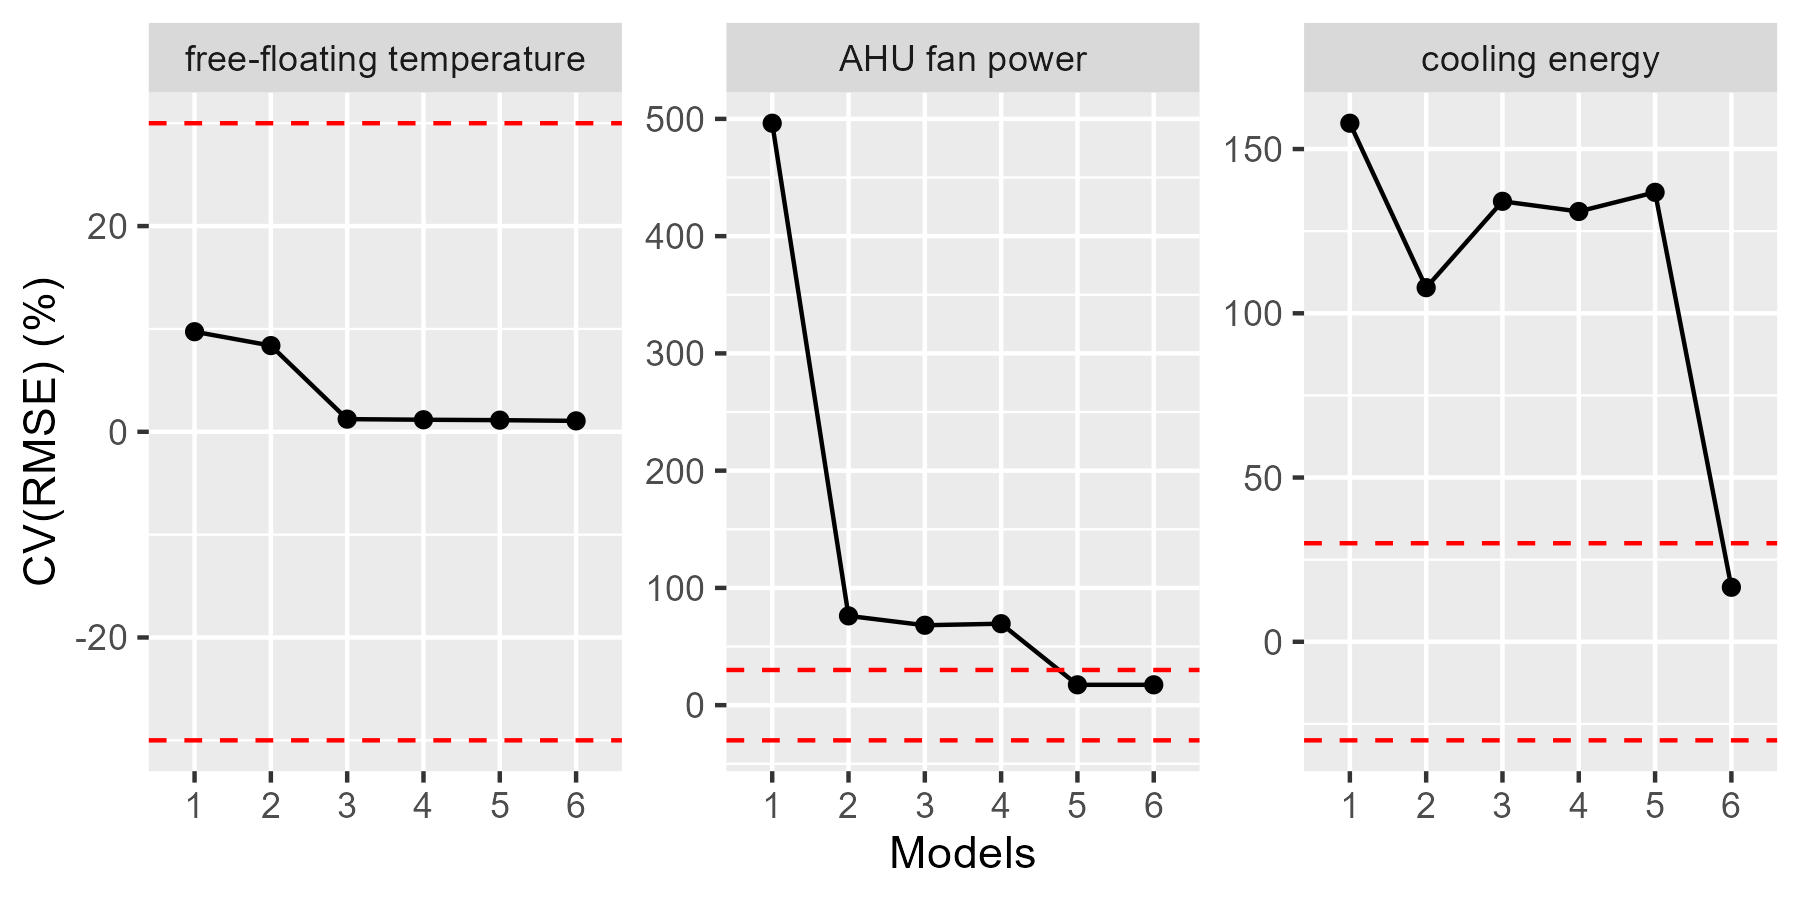
\includegraphics[width=1\linewidth]{pic/calibration_level_accuracy.jpg}
\caption{Results of CV(RMSE) in 1) free-floating temperature, 2) AHU fan power, and 3) cooling energy by the level of information. The red dotted lines denote the $\pm$30\% error limits specified in ASHRAE Guideline 14 \cite{guideline200214} for hourly CV(RMSE).}
% \caption{The evolution of CV(RMSE) from Level 1 to Level 6}
\label{fig:level_accuracy}
\end{figure}


\subsection{Different levels of information on ECM ranking and energy saving predictions}
\label{S:3.2}

Figure \ref{fig:bestoption_AC} illustrates the ranking of the five Energy Conservation Measures (ECMs) in AC mode. It is apparent that models established with LOIs 1 and 2 (no measurement data) result in a biased ranking of these ECMs. However, models established with LOIs 3, 4, and 5 can produce the same ECM ranking results as LOI 6 despite their limited additional information and lower accuracy in data fit compared to LOI 6. 

\begin{figure}[H]
\centering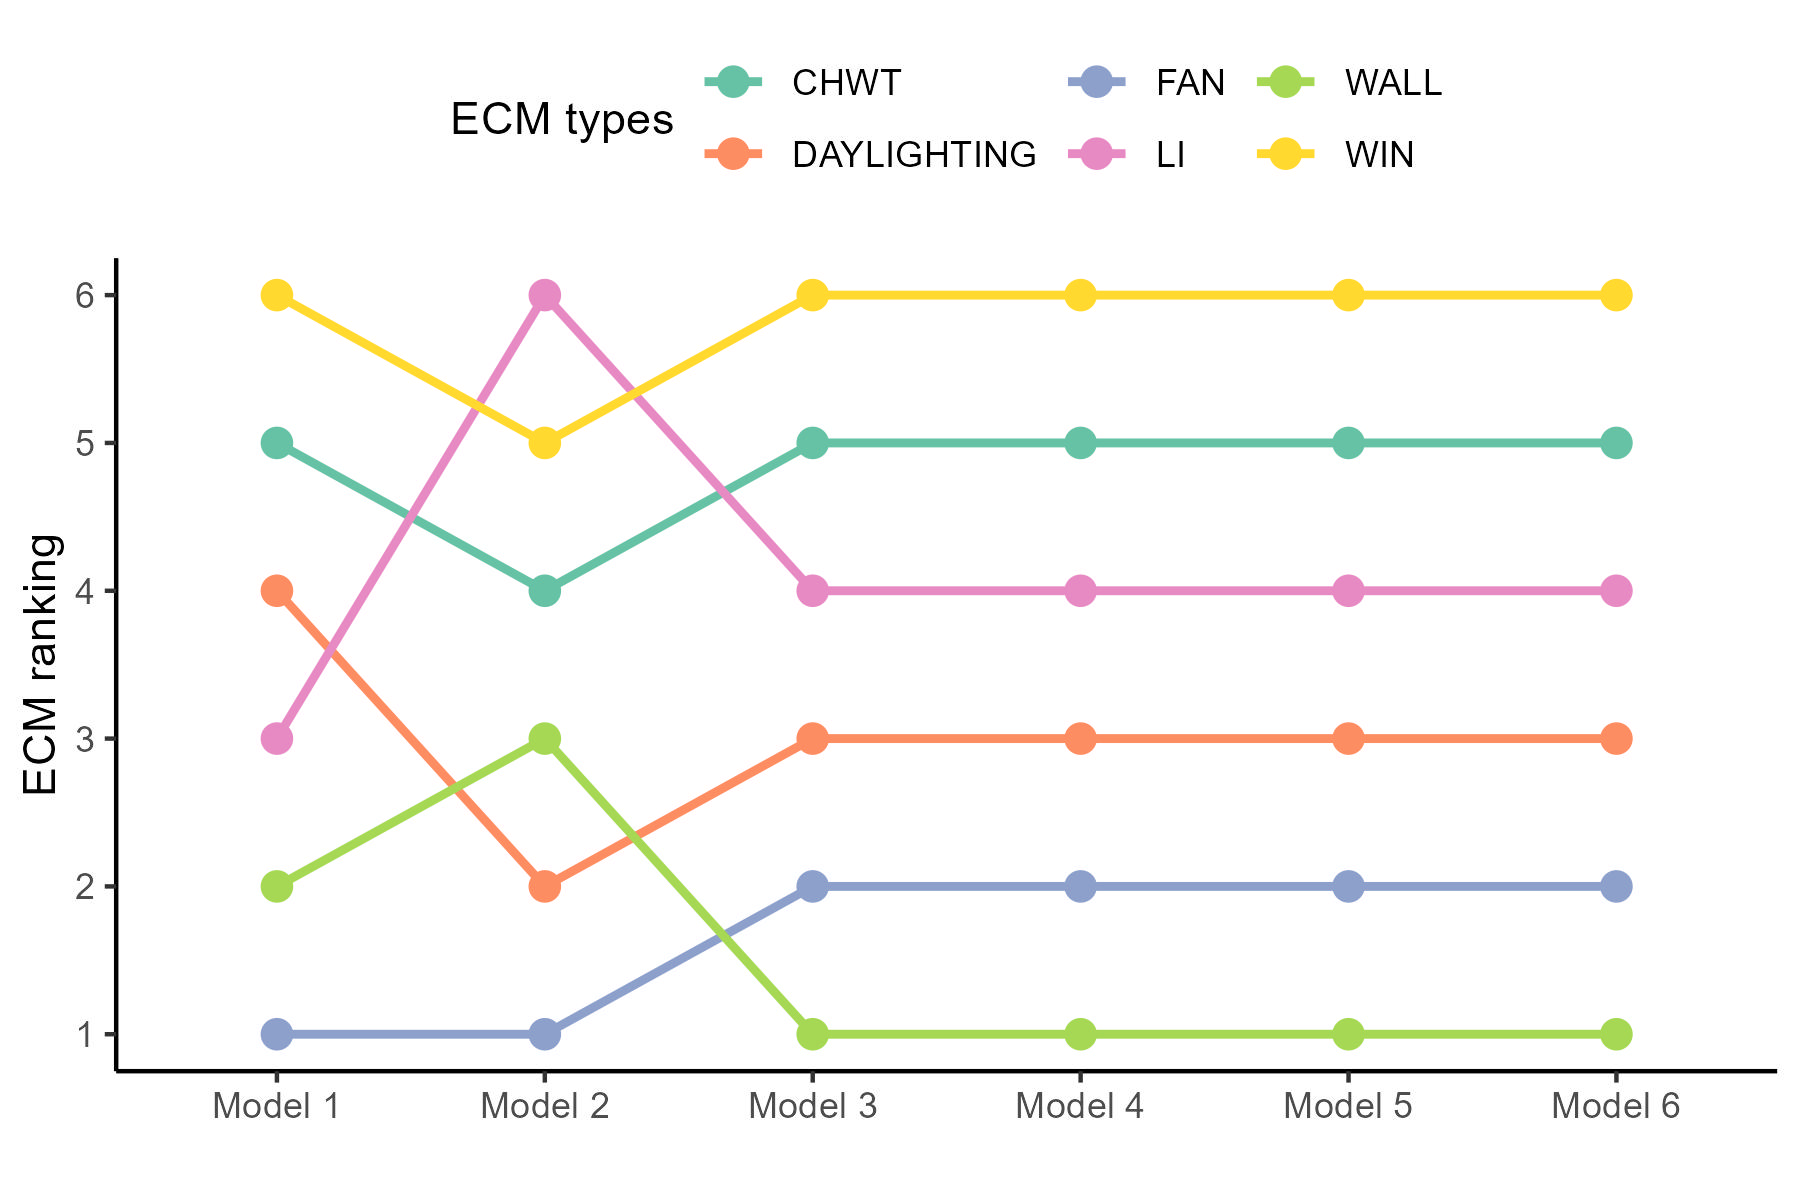
\includegraphics[width=0.85\linewidth]{pic/ECM_ranking_AC.jpg}
\caption{Comparison of the predicted ECM rankings under AC mode across different levels of information}
\label{fig:bestoption_AC}
\end{figure}

Figure \ref{fig:savings_AC} compares the percentage difference in estimated energy savings for each ECM to the predictions of Model 6. Noticeable variations in energy-saving predictions are observed for Models 1 and 2 compared to Model 6, ranging from a -90\% deviation to approximately tenfold (1000\%). Additionally, it is noticeable that although Models 3 to 5 manage to maintain a consistent ECM ranking aligned with Model 6, they fall short in terms of accuracy for energy-saving analysis, introducing a percentage difference ranging from -69\% to 94\% compared to Model 6's predictions.

\begin{figure}[H]
% \centering\includegraphics[width=1\linewidth]{pic/ECM_savings_AC_2.jpg}
\centering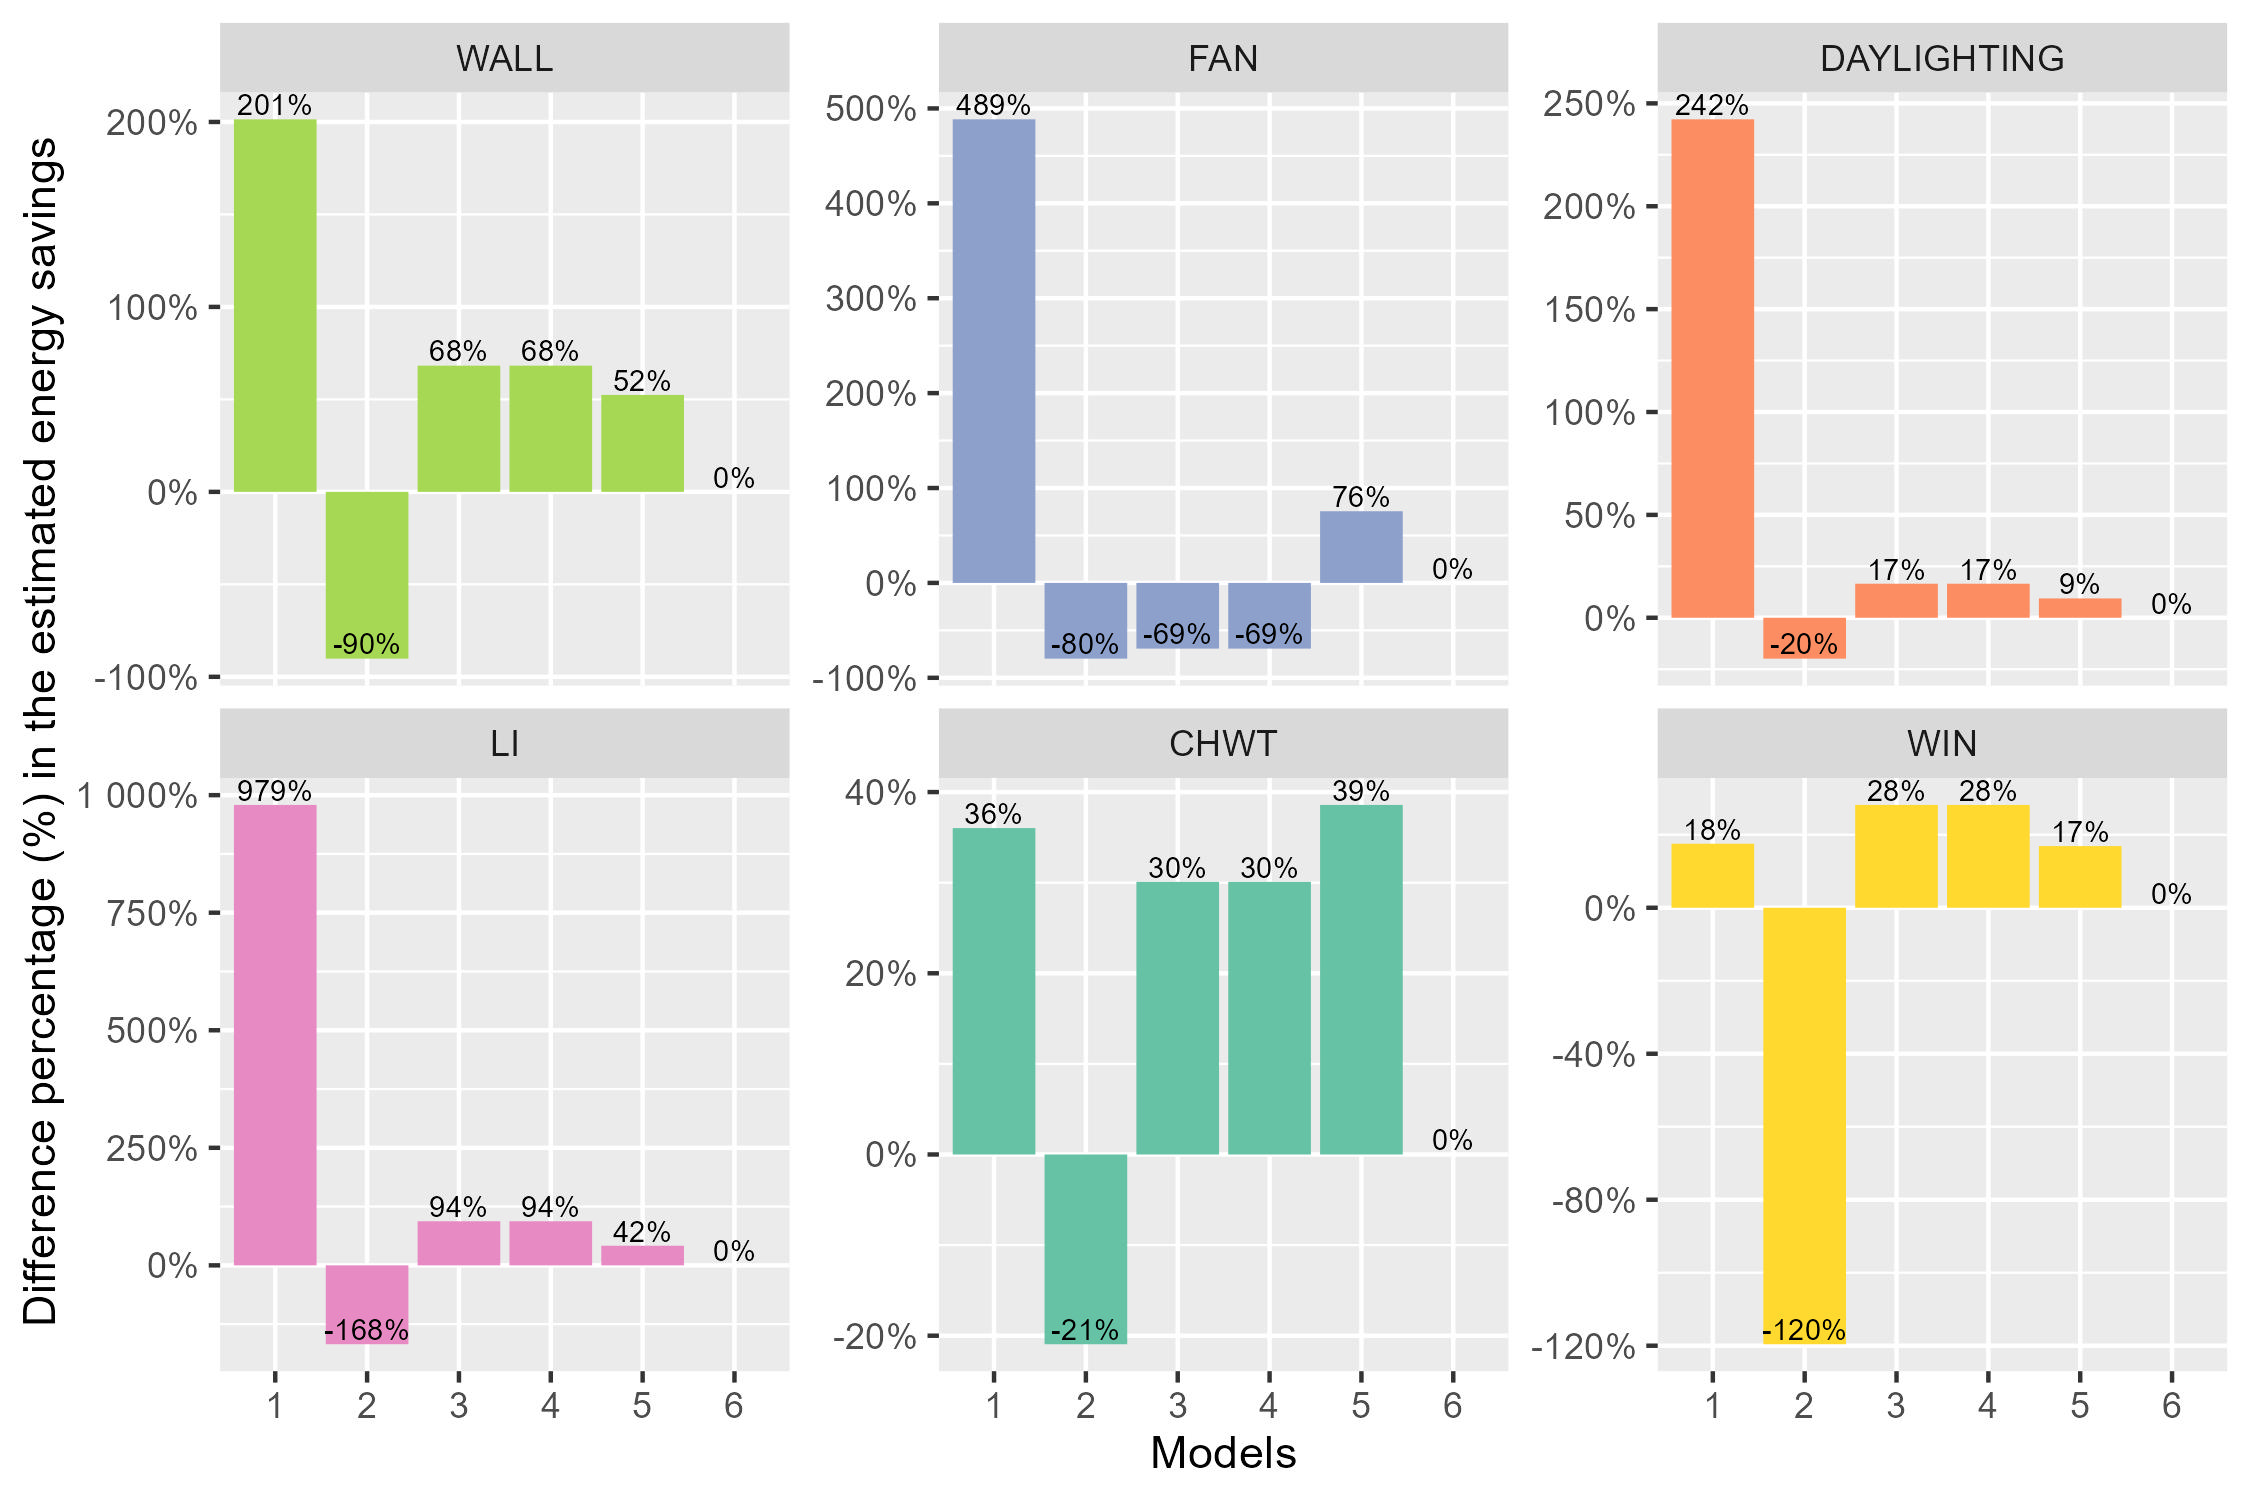
\includegraphics[width=1\linewidth]{pic/savings_diff_percentage_AC.jpg}
\caption{Comparison of estimated energy savings under AC mode across different levels of information}
\label{fig:savings_AC}
\end{figure}


\subsection{Results under mixed-mode conditions}
\label{S:3.3}

The ECM ranking results under mixed-mode ventilation (MMV) are shown in Figure \ref{fig:bestoption_MM}. It can be seen that Models 3 to 5 have slightly different ECM rankings compared to Model 6. This result indicates that the models operating at mixed-mode conditions need more input information to calibrate the model better to represent the building performance under dynamic operation conditions. It was also observed that compared with Models 1 and 2, Models 3 to 5 developed ECM rankings much closer to Model 6, manifesting an improved predictive performance for ECM ranking due to the increased information for calibration.

\begin{figure}[H]
\centering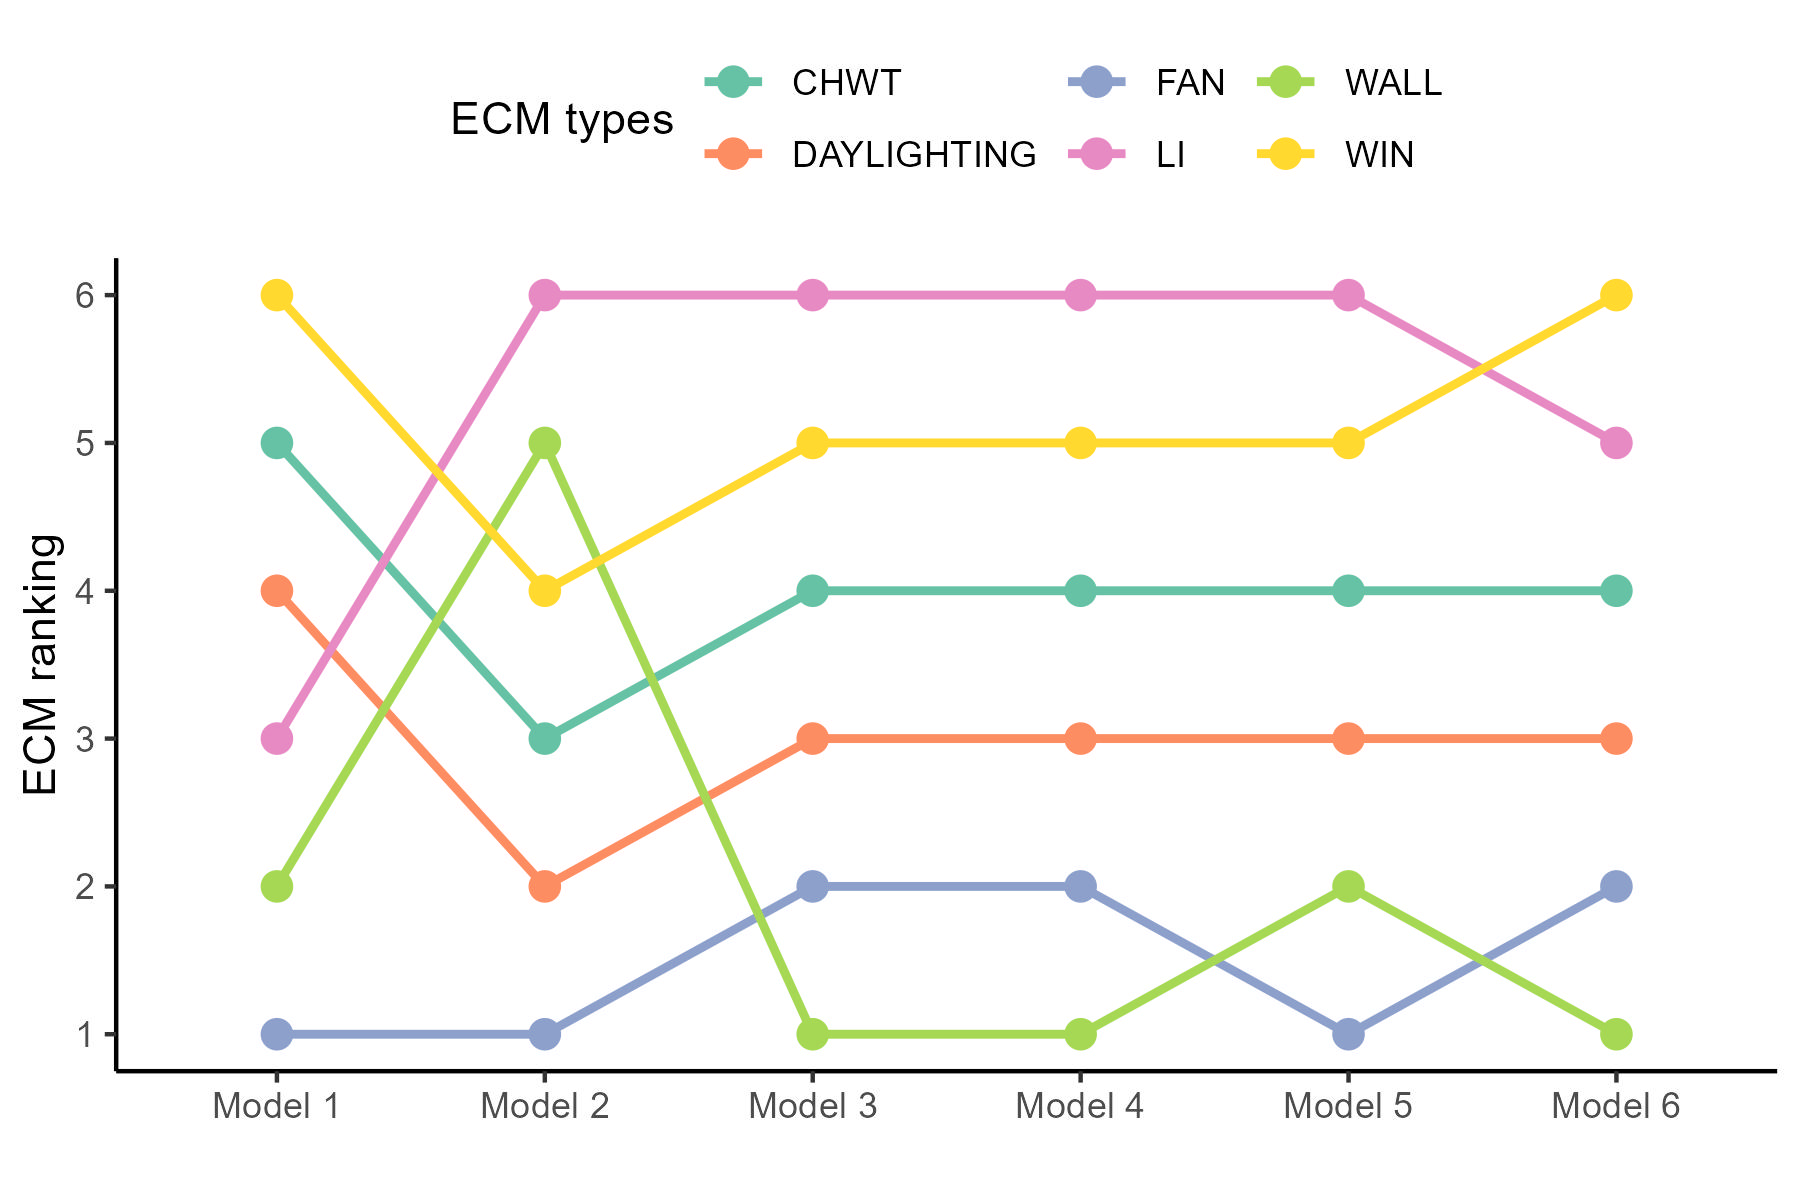
\includegraphics[width=0.85\linewidth]{pic/ECM_ranking_MM.jpg}
\caption{Comparison of the predicted ECM rankings under MM (mixed-mode) across different levels of information}
\label{fig:bestoption_MM}
\end{figure}

The above results (as shown in Figure \ref{fig:bestoption_MM} and \ref{fig:bestoption_AC}) suggest that the calibrations from Model 3 onwards can identify the top two energy-efficient ECMs for all cases. Obviously, these levels exhibit much better predictive performance for ECM ranking than Model 1 and Model 2 in AC and MMV scenarios. This improvement may be attributed to the inclusion of envelope thermal conductivity measurements, which significantly enhances the model's representation of thermal dynamics, particularly in terms of building cooling load. The cooling load profiles shown in Figure \ref{fig:cooling_loads} for Model 1 to Model 6 underscore this enhancement. It is evident that, compared to Models 1 and 2, there is a notable improvement in the representation of the cooling load profile from Model 3 onward. This improvement provides a foundation for the enhanced consistency of ECM rankings with Model 6 for all ECMs from Model 3 onward. 

\begin{figure}[H]
\centering\includegraphics[width=1\linewidth]{pic/designday_clgload.jpg}
\caption{Design day cooling load profiles of the case studied building for different levels of information}
\label{fig:cooling_loads}
\end{figure}
% derived from the building energy simulation models calibrated from Level 1 to Level 6

Figure \ref{fig:savings_MM} compares the performance for different levels of information for each ECM under AC and MMV scenarios. The estimated energy savings for Model 1 were excluded from the visual plots due to their higher deviation than other levels. The colored lines in each plot represent different ECM options, and the triangular dots denote the first-ranking options among the ECMs. The dotted lines in each plot denote a ±30\% difference from Model 6's energy-saving estimate as a reference. It is clear that the increased level of information does not consistently reduce errors in predicted ECM energy savings. The performance of different information levels varies across ECMs and operation modes. In general, the estimated energy savings of the ECMs exhibit the most significant variations when the specific level of information directly related to that ECM is introduced. For example, incorporating measured thermal conductivity in Model 3 leads to a more significant change in estimated energy savings for WALL and WIN measures compared to the introduction of measurement information in other levels. Similarly, adding fan power measurements and tuning fan part load curve in Model 5 results in a more substantial change in estimated energy savings for FAN measures than other levels. These results highlight the importance of incorporating information directly related to the Quantity of Interest (QOI) based on the Context of Use (COU) (which is retrofit analysis in this study). 

\begin{figure}[H]
% \centering\includegraphics[width=1\linewidth]{pic/savings_diff_percent_both}
\centering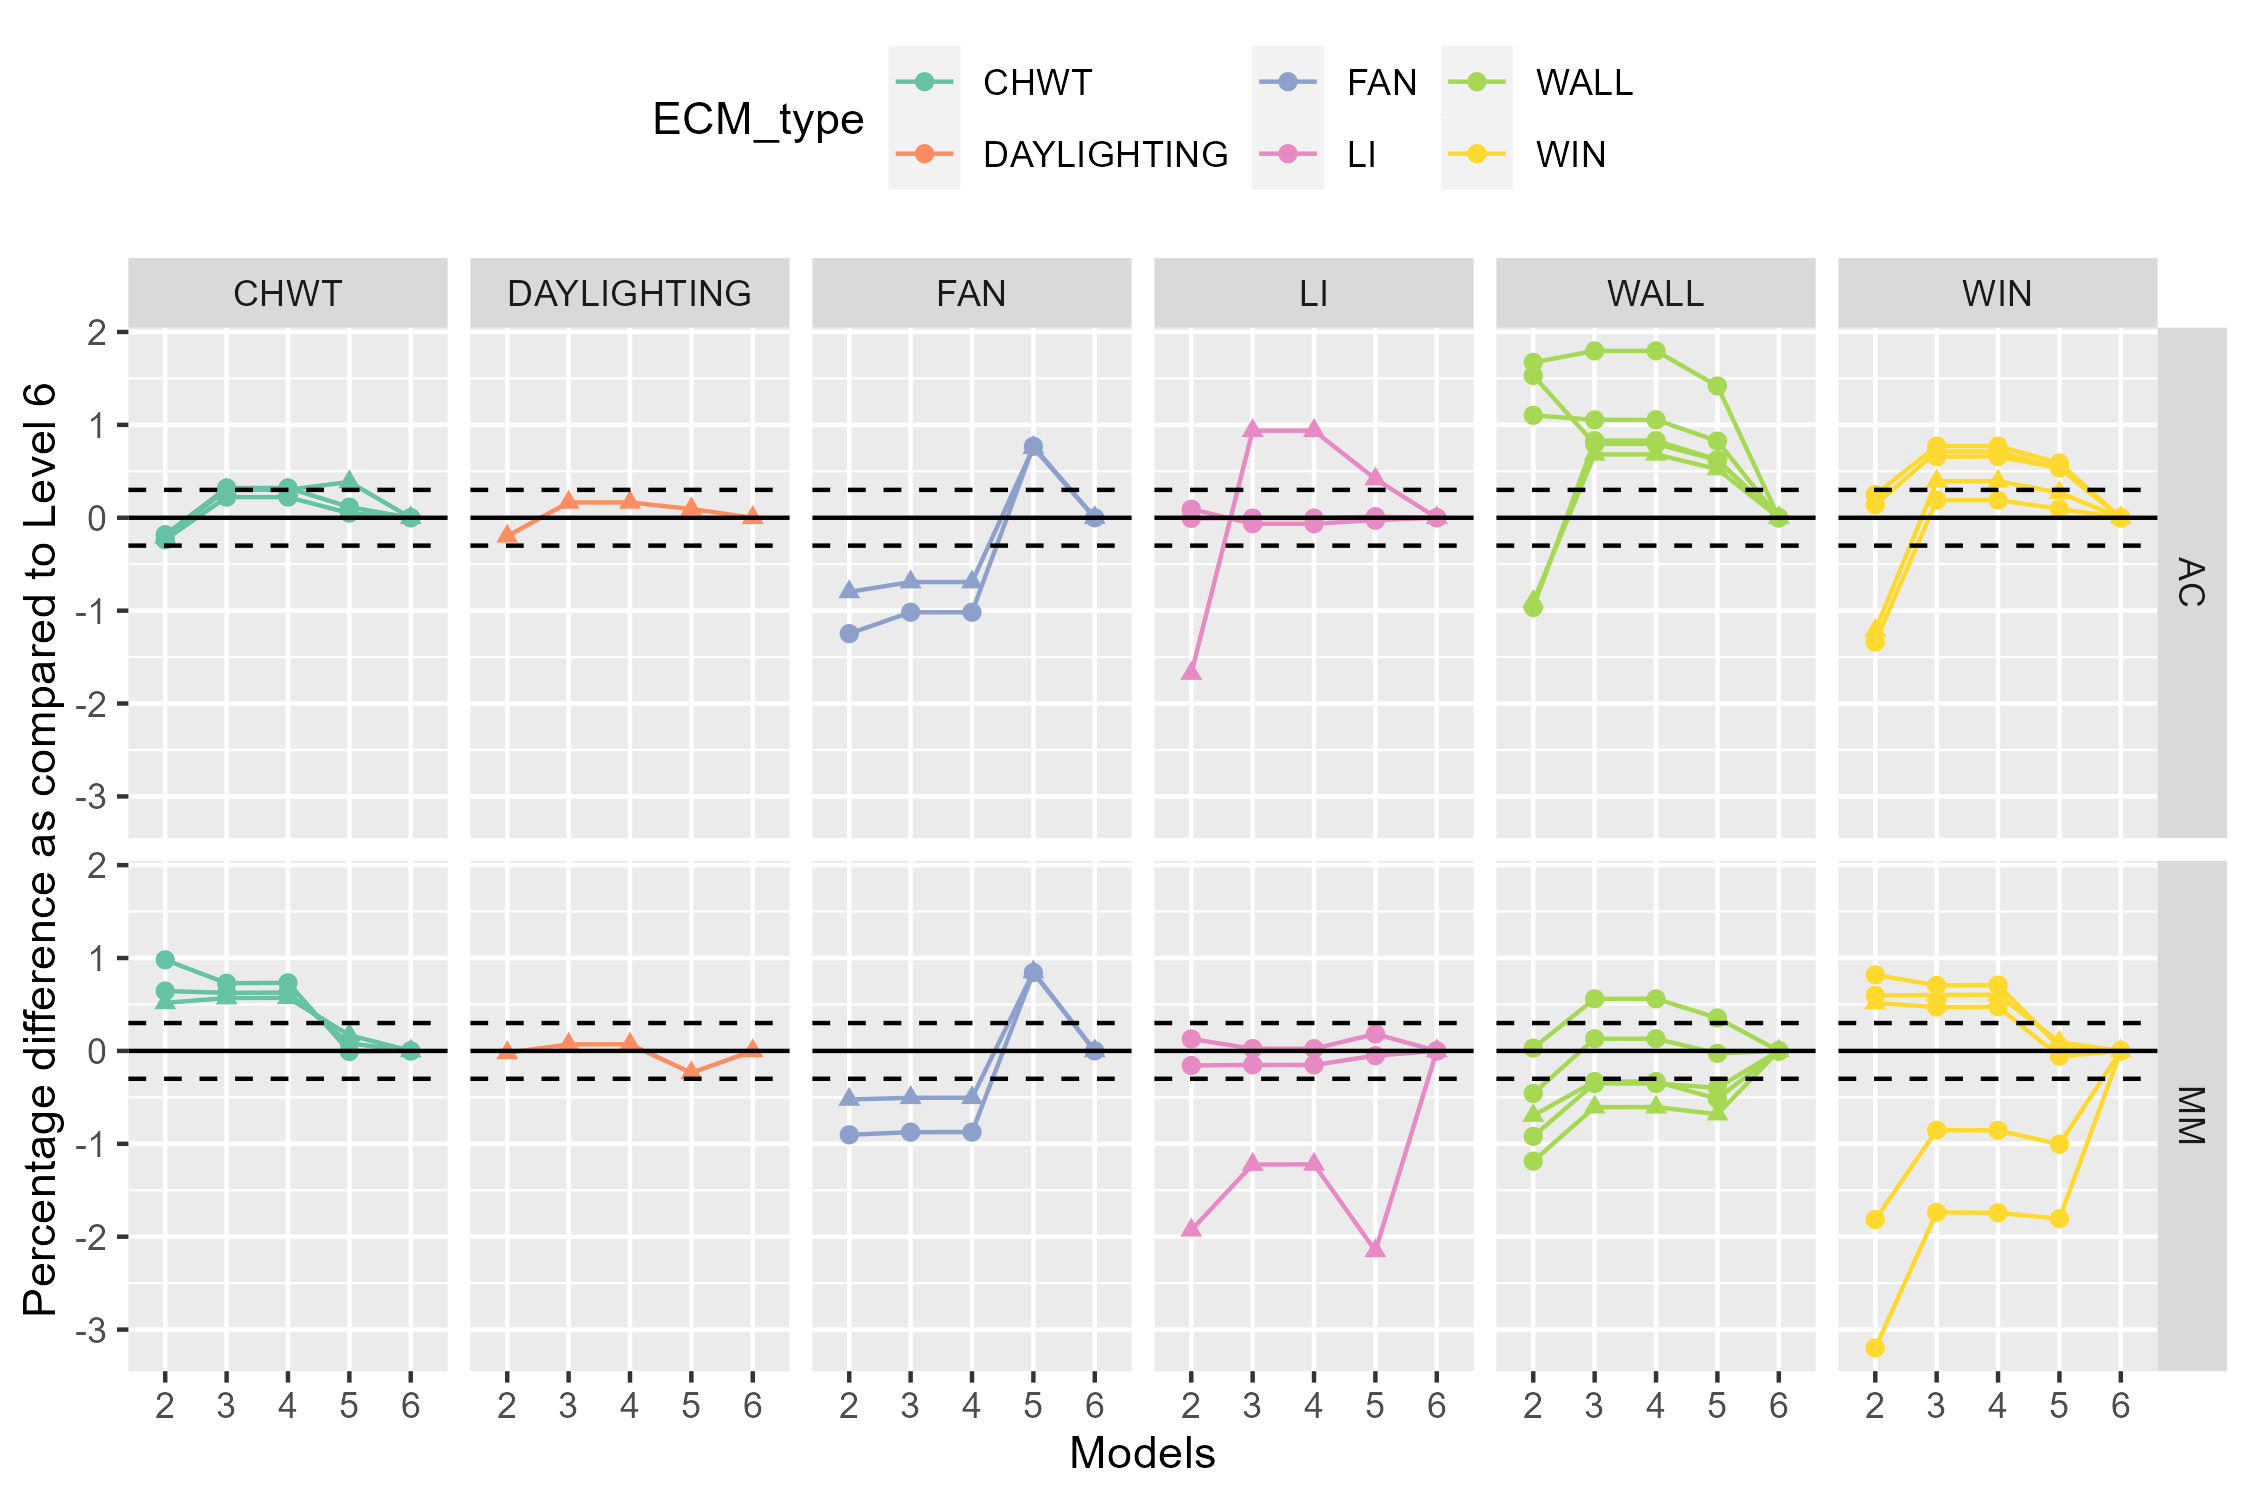
\includegraphics[width=1\linewidth]{pic/energy_saving_percent_line5.jpg}
\caption{Variation of the percentage difference from Model 2 to Model 6 under AC and MMV scenarios. The percentage difference is the difference in estimated energy savings between Model 6 and the remaining levels divided by Model 6's energy-saving predictions. The dotted lines denote a ±30\% difference from Model 6's estimate as a reference.}
\label{fig:savings_MM}
\end{figure}

Another notable observation from Figure \ref{fig:savings_MM} is that, for energy-saving predictions, the level of information has a significant impact on the modeled results. Specifically, taking the predictions of Model 6 as a reference, \textbf{the addition of design information} based on as-built documents and on-site verification (LOI 2) results in the most substantial difference in estimated energy savings, ranging from a decrease of -437.8\% (first quartile) to an increase of 12.1\% (third quartile). Following closely, \textbf{deriving the fan operational curve of part-load performance} (LOI 5) introduces considerable variance in predicted energy savings, with a first-quartile decrease of -50.8\% and a third-quartile increase of 118.7\%. Additionally, \textbf{tuning the minimum outdoor air fraction} (Model 6) can lead to a first-quartile decrease of -71.0\% and a third-quartile increase of 2.8\% in energy-saving predictions. \textbf{The addition of envelope thermal property measurements} (LOI 3) also exerts influence, causing the estimated energy savings to range from a decrease of -29.7\% (first quartile) to an increase of 61.0\% (third quartile). In contrast, the measured infiltration rate (LOI 4) has minimal impact on the models' energy-saving predictions, with the average difference in the percentage of total energy consumption between Models 3 and 4 being less than 1\%.

Furthermore, the results show that except for the CHWT and DAYLIGHTING measures, the energy savings estimated from Model 5 for the remaining ECMs all exceed a ±30\% range of difference compared to estimations from Model 6. The substantial variation in estimated energy savings, even at Model 5, implies that the model, calibrated against two data streams (free-floating temperature and AHU fan power on an hourly basis in this case), is insufficient for a robust prediction of ECM relative savings. Consequently, for energy-saving predictions, it is recommended that the model be calibrated against all outputs of interest using available information collected within the acceptable range of calibration efforts.


\section{Discussions}
\label{S:4}

\subsection{Towards simultaneous accuracy for multiple outputs}
\label{S:4.1}
The results of this study emphasize that providing a specific level of information can only enhance the predictive accuracy of outputs closely linked to that information. Therefore, a model well-calibrated against one output may not give accurate predictions for other outputs. This provides empirical evidence for the non-identifiability issue. Given the complex system dynamics and heterogeneous building characteristics, a considerable amount of information would be needed to achieve simultaneous accuracy at multiple levels.

However, the lack of measurements and detailed information for calibration is common in digital twin modeling. According to a recent review on calibrating building energy simulation models \cite{chong2021calibrating}, more than 90\% of the reviewed papers calibrated the model against a maximum of one (62\%) or two (29\%) outputs, and only 1\% performed the calibration using over three outputs. An overview of 51 urban building energy modeling studies \cite{oraiopoulos2022accuracy} shows that 20 out of 51 digital twins for UBEM did not specify any measured data for calibration, and 30 out of 51 are calibrated against the energy consumption data in annual resolution. A critical question arises: Whether these digital twins are true representations that accurately mirror their physical counterparts and inform decisions that realize value? Additionally, many automatic calibration tools are proposed to ease the user into tuning a wide range of “uncertain” parameters to achieve a good data fit using advanced algorithms and supercomputers. For example, an automatic calibration tool developed by the Oak Ridge National Laboratory was reported to be able to autotune 156 EnergyPlus inputs in three hours to match either monthly or hourly electrical usage within error limits \cite{garrett2015scalable}. However, whether the single data stream is informative enough for calibrating so many parameters remains unanswered. These questions emphasize the need for more studies into a sufficient level of information for a simulation model that is compatible with its intended purpose.


\subsection{Towards reliable predictive performance}
\label{S:4.2}
Developing a building energy model with high accuracy requires substantial effort for information and data gathering. However, the reliability of a model for its intended purpose, particularly in retrofit analysis, is not solely contingent on its accuracy. As the statistician George Box pointed out, “All models are wrong, but some are useful.” The model's reliability depends on its context of use. The results of this study show that a model that did not meet the accuracy limits specified in ASHRAE Guideline 14 \cite{guideline200214} might give correct retrofit decisions in terms of ECM ranking as long as it could capture the peak cooling load profile in simulation. Therefore, a calibration with envelope thermal measurements is necessary for ECM ranking analysis. However, for energy-saving analysis, the level of information can significantly affect the simulated energy savings. Thus, it is necessary to calibrate the model against all outputs of interest with sufficient information for more reliable and trustworthy energy-saving projections. The findings from this study are contrary to previous studies that have used uncalibrated models to simulate and analyze building energy savings \cite{ye2021evaluating, sun2017framework, heo2015scalable}. We demonstrated that uncalibrated models are unreliable both in absolute accuracy and in relative comparison. Calibration is a necessary and crucial step in the search for parsimonious models compatible with their intended purpose.

\subsection{The misuse of accuracy metrics}
\label{S:4.3}
The findings underscore the limited effectiveness of CV(RMSE) in evaluating calibration performance for its intended purpose. Specifically, we demonstrate that a model with a high CV(RMSE) value can still yield correct ECM ranking for retrofit decisions. In contrast, a low CV(RMSE) does not indicate a good model, as a good data fit for one output does not ensure the simulation model's precision in predicting other outputs due to identifiability issues. Limitations of the accuracy metrics stem from their inherent characteristics. The statistical basis of ASHRAE Guideline 14's accuracy criteria lies in a graphical calibration method proposed by \citet{reddy1997baselining}. This methodology employs CV(RMSE) to evaluate the goodness-of-fit of a regression model. Hence, the accuracy limits specified in ASHRAE Guidelines are designed for a statistical/correlational (black-box) model and cannot be directly applied to the dynamic simulation (white-box) model. \citet{reddy2000uncertainty} pointed out that absolute cutoff criteria may not be appropriate since no clear rationale for their choice is provided. The limitations of statistical indices in calibration performance evaluation justify the necessity of incorporating empirical evidence \cite{homer2014levels} and emphasizing the principle of equifinality \cite{beven2001equifinality} in modeling and calibration. If one can model the quantity of interest with the minimum level of information based on observed evidence in the building, credible modeling can be achieved without over-tuning the models to meet a predefined accuracy threshold.

\subsection{Limitations and further research}
\label{S:4.4}
The study employed an evidence-based sequential calibration framework guided by expert knowledge and information hierarchy to assess the impact of different levels of information on building energy model calibration. While this framework forms a solid basis for the evaluation, it introduces limitations, restricting calibration parameters and offering little flexibility in the calibration sequence. For instance, the study does not explore the effect of each level of information only on the model's predictive performance. In addition, questions regarding the outcome of combining each level of information with tuning the parameters outside the provided information are not studied. Addressing these questions falls beyond the study's scope. However, in future work, we will integrate an optimization-based calibration process into the sequential framework and investigate the impact of different levels of information within the new framework. This would allow investigation into whether blind tuning can enhance lower levels of information to achieve calibrated models with satisfactory performance, comparable to models calibrated with more comprehensive information.

Another weakness is that the case study is a single-zone test bed located in Singapore. Observations regarding the dependence on the level of information may not fully represent multi-zone buildings and buildings in other climate types. To improve the generalizability and robustness of the findings developed from this study, future research will extend testing across diverse climates, building types, and application contexts while accounting for input uncertainties.

Last but not least, a more in-depth analysis is needed to demonstrate the effects of different levels of information on the model’s predictive performance. Quantitative methods, such as information theory, are worth exploring to elaborate the relationship between added information and observed outputs and explain how varying levels of information impact calibration performance regarding the simulation purpose.


\section{Conclusions}
\label{S:5}

Most existing studies have focused on the automation of the calibration process, often with the aim of minimizing errors between predictions of the simulation output and measured data. However, the impact of information on building energy model estimation is largely overlooked. Many studies have revealed that incorporating more information in the modeling process can increase calibration accuracy, such as \cite{kim2016stepwise}, \cite{de2018impact}, \cite{lim2018influences}, \cite{risch2021influence}. Nonetheless, not many works have been carried out to quantify the impact of different levels of information on a model's predictive performance for a specific context of use.  

To address this gap, we model and calibrate a test bed with different levels of information. Starting with an initial model based on building geometry (LOI 1), we gradually introduce additional information, including nameplate information (LOI 2), envelope conductivity (LOI 3), zone infiltration rate (LOI 4), AHU fan power (LOI 5), and HVAC data (LOI 6). Models with different levels of information were then applied for retrofit analysis across six ECMs under two operating conditions. The evaluation is performed with standardized accuracy-based metrics and performance evaluation on the models' ECM ranking and energy-saving estimations. The key findings of the study can be summarized as follows:

\begin{itemize}
\item \textbf{Calibration accuracy}: Incorporating more information in the calibration process leads to an improved fit between the simulation and measured data. However, this improvement is not uniform across all observed outputs. The accuracy of specific observed output is improved only when additional information directly linked to that output is introduced and specified in the building energy model. Therefore, reliable calibration is contingent on gathering information closely correlated with the outputs of interest, particularly when simultaneous accuracy for multiple outputs is necessary. 
\item \textbf{Predictive performance for ECM ranking}: Results from the case study show that for ECM ranking, models with low information and high CV(RMSE) values can still give correct retrofit decisions. It suggests a minimum calibration with envelope thermal measurements is necessary for ECM ranking.
\item \textbf{Predictive performance for energy savings}: Predictive performance in terms of energy savings is profoundly influenced by the level of information used in calibration. In contrast to Model 6, which is calibrated against measured free-floating temperature, AHU fan power, and cooling energy, ECM energy-saving predictions exhibit substantial differences in other models. Model 1, the uncalibrated model, shows variations of up to ten times (1000\%). Model 3, calibrated against measured free-floating temperature, displays variances of up to 180\%, while Model 5, calibrated against measured free-floating temperature and AHU fan power, shows a deviation of up to -215\%.
\end{itemize}

The results from this study highlight the limitations of CV(RMSE) in characterizing the validity of calibration for its intended purpose. A low CV(RMSE) for a specific output is not indicative of good calibration, as it does not guarantee simultaneous accuracy for all outputs of interest. In contrast, a model that did not meet ASHRAE 14 accuracy thresholds might still be reasonable for its intended purpose. Therefore, instead of adhering to predefined accuracy thresholds, it is important to investigate the influence of different levels of information on the validity and reliability of building energy model calibration. The findings also indicate that the uncalibrated models are not reliable both in absolute accuracy and in relative comparison. Calibration is a necessary and crucial step in the search for parsimonious models compatible with their intended purpose. In summary, to balance the efforts for information-gathering and model reliability, it is crucial to 1) determine the minimum level of information required to achieve a simulation model that is compatible with its intended purpose and 2) calibrate models with information that is closely linked to the outputs of interest particularly when simultaneous accuracy for multiple outputs is necessary.

% ----------------------------------------------------------------------------------
% \section{Acknowledgements}
% This research project is supported by the National Research Foundation, Singapore, and Ministry of National Development, Singapore under its Cities of Tomorrow R\&D Programme (CoT Award COT-V4-2020-5); the National Research Foundation, Prime Minister's Office, Singapore under its Campus for Research Excellence and Technological Enterprise (CREATE) program through a grant to the Berkeley Education Alliance for Research in Singapore (BEARS) for the Singapore-Berkeley Building Efficiency and Sustainability in the Tropics (SinBerBEST) Program. 
% ----------------------------------------------------------------------------------
% \section*{Data availability} \label{sec:open}
% The research compendium for this article can be found at \url{https://github.com/ideas-lab-nus/sbb-calibration}, hosted at GitHub.

% TC:ignore
% ----------------------------------------------------------------------------------
% \section*{CRediT authorship contribution statement}
% \textbf{Siyu Cheng:} Methodology, Formal analysis, Investigation, Data curation, Visualization, Writing – Original Draft.
% \textbf{Zeynep Duygu Tekler:} Visualization, Writing - Review \& Editing. 
% \textbf{Hongyuan Jia:} Investigation, Data Curation, Writing - Review \& Editing. 
% \textbf{Wenxin Li:} Investigation, Data Curation.
% \textbf{Adrian Chong:} Conceptualization, Methodology, Writing - Review \& Editing, Supervision, Project administration, Funding acquisition.
% ----------------------------------------------------------------------------------

\bibliography{reference} % ref
\bibliographystyle{elsarticle-num-names}

\begin{appendices}
\section{Appendix}

\setcounter{figure}{0} 

\renewcommand{\figurename}{Figure}
\renewcommand{\thefigure}{A\arabic{figure}}

\begin{figure}[H]
\centering\includegraphics[width=0.9\linewidth]{pic/FF_Tair_verify_new.jpg}
\caption{Measured and predicted hourly indoor air temperatures [$ ^\circ C $] under free-floating}
\label{fig:temperature}
\end{figure}

\begin{figure}
\centering\includegraphics[width=0.9\linewidth]{pic/fan_power_new.jpg}
\caption{Measured and predicted fan energy power [W] at an hourly resolution}
\label{fig:fan_power}
\end{figure}

\begin{figure}
\centering\includegraphics[width=0.9\linewidth]{pic/CHW_Clg_rate_new.jpg}
\caption{Measured and predicted chilled water cooling rate [W] at an hourly resolution}
\label{fig:cooling_rate}
\end{figure}

\end{appendices}


\end{sloppypar}
\end{document}
